\section{Statistical modelling of CPU forward and backward passes}
\label{sec:chaining-runl-repeat-experiment}
\label{sec:chaining-cpu-experimental-analysis}

The first loop in Algorithm~\ref{alg:chaining-simd-backtrack} can process
\(L\) anchors at once only when \(\operatorname{Run}_L(j,c)\) is true. 
We also use update counter $U$ in Algorithm~\ref{alg:chaining-b5} to terminate loop if the consecutive updates don't improve any SIMD lane.
At the same time minimap2 uses \text{max\_drop} in its algorithm~\ref{fig:chaining-minimap2-backtracking} to terminate backtracking if the score drop is too large.

We never explained any proper justification for using or not using these heuristics. This section talks about random synthetic data and intuitive explanation behind the choices.
The subsections talk about:
\begin{itemize}
  \item Preparing synthetic data (randomly generated sequences with insertions/deletions) and specially constructed examples aimed at absuing the scoring function and thresholds
  \item Answering if counting number of updates that do not improve score in forward chaining algorithm~\ref{alg:chaining-b5} improve performance
  \item Answering if the anchors during backtracking~\ref{alg:chaining-simd-backtrack} are just continous sequences of indices incremented by 1 (\(\operatorname{Run}_L(j,c)\) condition)
  \item Answering if max drop would help us increase performance of SIMD backtracking algorithm or not~\ref{fig:chaining-minimap2-backtracking}
\end{itemize}

\warn{Synthetic data}{Primary modelling here uses synthetic
data built from randomly generated sequences assuming default substitution rate of $0.001$ and insertion/deleteion probability of $0.0005$. I prepared special cases of sequence construction using gaps or equal regions to see what happens in cases where extremally large gaps occur as secondary method of analysis. Overall the analysis is intended to
motivate the approach and formulate conditions under which an optimisation's
cost exceeds its benefit.}

\subsection{Problematic chains}

As mentioned in section~\ref{sec:chaining-interpretation} there is a case of emergent assymetry: if one anchor matches with multiple anchors in the query, then we cannot easily tell which part of the query is best to match. The following sections demonstrates what happens in this scenario. The special query/target constructions are prepared in that asymmetry in mind.


\subsubsection{Reference and query structures}

\begin{figure}[p]
\centering
\begin{tikzpicture}[
  x=1cm,y=1cm,font=\scriptsize,>=Latex,
  runl unit/.style={
    draw=black!60,minimum height=.48cm,align=center,
    inner sep=1.5pt,outer sep=0pt,rounded corners=0pt},
  runl unique/.style={
    runl unit,draw=chainGray!85!black,fill=chainGray!10},
  runl source/.style={
    runl unit,draw=chainBlue!90!black,fill=chainBlue!13},
  runl variant/.style={
    runl unit,draw=chainOrange!95!black,fill=chainOrange!16},
  runl selected/.style={
    runl unit,draw=chainGreen!80!black,fill=chainGreen!14,very thick},
  runl unused/.style={
    runl unit,draw=chainOrange!95!black,fill=chainOrange!10,dashed},
  runl cell/.style={
    runl unit,minimum width=.52cm,minimum height=.42cm,
    fill=chainGray!8,font=\tiny},
  runl chosen cell/.style={
    runl cell,draw=chainGreen!80!black,fill=chainGreen!16,very thick},
  runl gap/.style={
    runl unit,draw=black!35,fill=black!3,minimum height=.36cm,
    inner sep=.6pt,font=\tiny},
  runl main/.style={line width=.85pt,draw=chainGreen!80!black},
  runl extra/.style={
    line width=.75pt,draw=chainOrange!95!black,dashed},
  runl pred/.style={-{Latex[length=1.4mm]},thick,draw=black!72},
  runl note/.style={
    draw=black!45,fill=black!2,align=left,
    inner sep=3pt,rounded corners=0pt},
  runl info/.style={
    runl note,text width=3.35cm,minimum height=1.60cm,font=\tiny}
]
  \node[anchor=west,font=\bfseries] at (.10,12.80)
    {(a) Mosaic};

  \node[anchor=east] at (.72,12.22) {reference};
  \node[runl unique,minimum width=.70cm] (mrUzero) at (1.25,12.22)
    {\(U_0\)};
  \node[runl source,minimum width=3.00cm] (mrA) at (3.15,12.22)
    {\(A\)};
  \node[runl unique,minimum width=.70cm] (mrUone) at (5.05,12.22)
    {\(U_1\)};
  \node[runl source,minimum width=3.00cm] (mrAprime) at (6.95,12.22)
    {\(A'=A\)};
  \node[runl unique,minimum width=.70cm] (mrUtwo) at (8.85,12.22)
    {\(U_2\)};

  \node[anchor=east] at (.72,11.52) {query};
  \node[runl unique,minimum width=.70cm] (mqUzero) at (1.25,11.52)
    {\(U_0\)};
  \node[runl source,minimum width=3.00cm] (mqA) at (3.15,11.52)
    {\(A\)};
  \node[runl unique,minimum width=.70cm] (mqUone) at (5.05,11.52)
    {\(U_1\)};
  \node[runl source,minimum width=3.00cm] (mqAprime) at (6.95,11.52)
    {\(A'=A\)};
  \node[runl unique,minimum width=.70cm] (mqUtwo) at (8.85,11.52)
    {\(U_2\)};

  \draw[runl main]
    (mrUzero.south)--(mqUzero.north)
    (mrA.south)--(mqA.north)
    (mrUone.south)--(mqUone.north)
    (mrAprime.south)--(mqAprime.north)
    (mrUtwo.south)--(mqUtwo.north);
  \draw[runl extra] (mrA.south)--(mqAprime.north);
  \draw[runl extra] (mrAprime.south)--(mqA.north);

  \node[runl info] at (11.75,11.87) {
    reference \(=\) query\\[2pt]
    \(A'=A\)\\
    \(\lvert A\rvert=\lvert A'\rvert=32768\) bp\\
    \(\lvert U_i\rvert=512\) bp\\
    block-start offset: \(33280\) bp
  };

  \draw[black!35] (.10,10.87)--(13.75,10.87);

  \node[anchor=west,font=\bfseries] at (.10,10.60)
    {(b) Degraded mosaic};

  \node[anchor=east] at (.72,10.02) {reference};
  \node[runl unique,minimum width=.70cm] (drUzero) at (1.25,10.02)
    {\(U_0\)};
  \node[runl source,minimum width=3.00cm] (drA) at (3.15,10.02)
    {\(A\)};
  \node[runl unique,minimum width=.70cm] (drUone) at (5.05,10.02)
    {\(U_1\)};
  \node[runl variant,minimum width=3.00cm] (drAprime) at (6.95,10.02)
    {\(A'_{\delta}\neq A\)};
  \node[runl unique,minimum width=.70cm] (drUtwo) at (8.85,10.02)
    {\(U_2\)};

  \node[anchor=east] at (.72,9.32) {query};
  \node[runl unique,minimum width=.70cm] (dqUzero) at (1.25,9.32)
    {\(U_0\)};
  \node[runl source,minimum width=3.00cm] (dqA) at (3.15,9.32)
    {\(A\)};
  \node[runl unique,minimum width=.70cm] (dqUone) at (5.05,9.32)
    {\(U_1\)};
  \node[runl variant,minimum width=3.00cm] (dqAprime) at (6.95,9.32)
    {\(A'_{\delta}\neq A\)};
  \node[runl unique,minimum width=.70cm] (dqUtwo) at (8.85,9.32)
    {\(U_2\)};

  \draw[runl main]
    (drUzero.south)--(dqUzero.north)
    (drA.south)--(dqA.north)
    (drUone.south)--(dqUone.north)
    (drAprime.south)--(dqAprime.north)
    (drUtwo.south)--(dqUtwo.north);
  \draw[runl extra] (drA.south)--(dqAprime.north);
  \draw[runl extra] (drAprime.south)--(dqA.north);

  \node[runl info] at (11.75,9.67) {
    reference \(=\) query\\[2pt]
    \(A'_{\delta}\neq A\)\\
    \(\lvert A\rvert=\lvert A'_{\delta}\rvert=32768\) bp\\
    \(\lvert U_i\rvert=512\) bp\\
    block-start offset: \(33280\) bp
  };

  \draw[black!35] (.10,8.67)--(13.75,8.67);

  \node[anchor=west,font=\bfseries] at (.10,8.40)
    {(c) Spaced copy};

  \node[anchor=east] at (.72,7.82) {reference};
  \node[runl source,minimum width=1.50cm] at (1.48,7.82) {\(S\)};
  \node[runl unique,minimum width=1.50cm] at (3.00,7.82) {\(N^G\)};

  \node[anchor=east] at (.72,7.15) {query};
  \node[runl source,minimum width=.78cm] at (1.10,7.15) {\(S_0\)};
  \node[runl unique,minimum width=.72cm] at (1.87,7.15) {\(N^G\)};
  \node[runl source,minimum width=.78cm] at (2.64,7.15) {\(S_1\)};
  \node[runl unique,minimum width=.72cm] at (3.41,7.15) {\(N^G\)};
  \node at (4.13,7.15) {\(\cdots\)};
  \node[runl source,minimum width=1.02cm] at (5.05,7.15)
    {\(S_{R-1}\)};
  \node[runl unique,minimum width=.72cm] at (5.95,7.15) {\(N^G\)};

  \node[runl info] at (11.75,7.47) {
    \(\lvert S_v\rvert=4096\) bp\\
    \(\lvert N^G\rvert=16384\) bp\\
    \(R\in\{1,2,4,8,16,32,64\}\)\\
    repeated-unit length: \(20480\) bp
  };

  \node[anchor=east] at (1.75,5.88) {\(r_t:\)};
  \node[runl cell] at (2.12,5.88) {\(0\)};
  \node[runl chosen cell] (previousV) at (2.70,5.88) {\(v\)};
  \node[runl cell] at (3.28,5.88) {\(R-1\)};

  \node[anchor=east] at (4.90,5.88) {\(r_{t+1}:\)};
  \node[runl cell] at (5.27,5.88) {\(0\)};
  \node[runl chosen cell] (currentV) at (5.85,5.88) {\(v\)};
  \node[runl cell] at (6.43,5.88) {\(R-1\)};

  \draw[runl pred]
    (currentV.north) .. controls +(0,.52) and +(0,.52) ..
    (previousV.north);
  \node[anchor=south,fill=white,inner sep=1pt] at (4.28,6.39)
    {\(p_j=j-R\neq j-1\quad(R\geq2)\)};
  \node[anchor=north] at (2.70,5.63) {index \(j-R\)};
  \node[anchor=north] at (5.85,5.63) {index \(j\)};

  \draw[black!35] (.10,5.15)--(13.75,5.15);

  \node[anchor=west,font=\bfseries] at (.10,4.88)
    {(d) Minimizer-island comb};

  \node[anchor=east] at (.72,4.30) {reference};
  \node[runl selected,minimum width=.44cm] (rP) at (1.02,4.30)
    {\(P\)};
  \node[runl gap,minimum width=.60cm] at (1.62,4.30)
    {\(N^{1475}\)};
  \node[runl unique,minimum width=.44cm] (rG) at (2.22,4.30)
    {\(G_t\)};
  \node[runl gap,minimum width=.60cm] at (2.82,4.30)
    {\(N^{1250}\)};
  \node[runl source,minimum width=.36cm] (rCzero) at (3.38,4.30)
    {\(c_0\)};
  \node[runl gap,minimum width=.65cm] at (3.97,4.30)
    {\(N^{3475}\)};
  \node[runl source,minimum width=.36cm] (rCone) at (4.55,4.30)
    {\(c_1\)};
  \node[runl gap,minimum width=.54cm] at (5.08,4.30)
    {\(N^{475}\)};
  \node[runl variant,minimum width=.46cm] (rRone) at (5.66,4.30)
    {\(R_1\)};
  \node[runl gap,minimum width=.60cm] at (6.27,4.30)
    {\(N^{1531}\)};
  \node[runl source,minimum width=.36cm] (rCtwo) at (6.83,4.30)
    {\(c_2\)};
  \node[runl gap,minimum width=.54cm] at (7.36,4.30)
    {\(N^{475}\)};
  \node[runl variant,minimum width=.46cm] (rRtwo) at (7.94,4.30)
    {\(R_2\)};
  \node[runl gap,minimum width=.60cm] at (8.55,4.30)
    {\(N^{1531}\)};
  \node[runl source,minimum width=.36cm] (rCthree) at (9.11,4.30)
    {\(c_3\)};
  \node at (9.55,4.30) {\(\cdots\)};

  \node[anchor=east] at (.72,3.63) {query};
  \node[runl selected,minimum width=.44cm] (qP) at (1.02,3.63)
    {\(P\)};
  \node[runl gap,minimum width=.54cm] at (1.59,3.63)
    {\(N^{975}\)};
  \node[runl unique,minimum width=.44cm] (qG) at (2.16,3.63)
    {\(G_q\)};
  \node[runl gap,minimum width=.54cm] at (2.73,3.63)
    {\(N^{975}\)};
  \node[runl source,minimum width=.36cm] (qCzero) at (3.26,3.63)
    {\(c_0\)};
  \node[runl gap,minimum width=.65cm] at (3.85,3.63)
    {\(N^{3375}\)};
  \node[runl source,minimum width=.36cm] (qCone) at (4.43,3.63)
    {\(c_1\)};
  \node[runl gap,minimum width=.44cm] at (4.91,3.63)
    {\(N^{25}\)};
  \node[runl variant,minimum width=.46cm] (qRone) at (5.44,3.63)
    {\(R_1\)};
  \node[runl gap,minimum width=.60cm] at (6.05,3.63)
    {\(N^{2081}\)};
  \node[runl source,minimum width=.36cm] (qCtwo) at (6.61,3.63)
    {\(c_2\)};
  \node[runl gap,minimum width=.54cm] at (7.14,3.63)
    {\(N^{925}\)};
  \node[runl variant,minimum width=.46cm] (qRtwo) at (7.72,3.63)
    {\(R_2\)};
  \node[runl gap,minimum width=.54cm] at (8.30,3.63)
    {\(N^{981}\)};
  \node[runl source,minimum width=.36cm] (qCthree) at (8.83,3.63)
    {\(c_3\)};
  \node at (9.27,3.63) {\(\cdots\)};

  \draw[runl main]
    (rP.south)--(qP.north)
    (rG.south)--(qG.north)
    (rCzero.south)--(qCzero.north)
    (rCone.south)--(qCone.north)
    (rRone.south)--(qRone.north)
    (rCtwo.south)--(qCtwo.north)
    (rRtwo.south)--(qRtwo.north)
    (rCthree.south)--(qCthree.north);

  \node[runl info] at (11.75,3.96) {
    spans: \(P=3925\) bp\\
    \(G_t=13525,\ G_q=9025\) bp\\
    \(c_k=25,\ R_k=1469\) bp\\
    \(R_k\) internal gap: 13 \(N\)\\
    horizontal distances are not to scale
  };

  \node[anchor=east] at (.72,2.31) {anchor array};
  \node[runl selected,minimum width=.82cm] (aP) at (1.18,2.31) {\(P\)};
  \node[runl selected,minimum width=.82cm] (aG) at (2.08,2.31) {\(G\)};
  \node[runl selected,minimum width=.58cm] (aCzero) at (2.82,2.31)
    {\(c_0\)};
  \node[runl selected,minimum width=.58cm] (aCone) at (3.50,2.31)
    {\(c_1\)};
  \node[runl unused,minimum width=.82cm] (aRone) at (4.30,2.31)
    {\(R_1\)};
  \node[runl selected,minimum width=.58cm] (aCtwo) at (5.10,2.31)
    {\(c_2\)};
  \node[runl unused,minimum width=.82cm] (aRtwo) at (5.90,2.31)
    {\(R_2\)};
  \node at (6.62,2.31) {\(\cdots\)};
  \node[runl selected,minimum width=.64cm] (aCm) at (7.35,2.31)
    {\(c_m\)};
  \node[runl selected,minimum width=1.08cm] (aRm) at (8.28,2.31)
    {\(e_m\in R_m\)};

  \draw[runl pred]
    (aRm.north) .. controls +(0,.28) and +(0,.28) .. (aCm.north);
  \draw[runl pred,dashed]
    (aCm.north) .. controls +(0,.60) and +(0,.60) .. (aCtwo.north);
  \draw[runl pred]
    (aCtwo.north) .. controls +(0,.60) and +(0,.60) .. (aCone.north);
  \draw[runl pred]
    (aCone.north) .. controls +(0,.28) and +(0,.28) .. (aCzero.north);
  \draw[runl pred]
    (aCzero.north) .. controls +(0,.28) and +(0,.28) .. (aG.north);
  \draw[runl pred]
    (aG.north) .. controls +(0,.28) and +(0,.28) .. (aP.north);

  \node[runl info] at (11.75,2.15) {
    first path:\\
    \(e_m\to\cdots\to r_{m,1}\to c_m\to\)\\
    \(\cdots\to c_0\to G\to P\)\\
    \(R_1,\ldots,R_{m-1}\): retained, off path
  };

  \draw[black!35] (.10,1.23)--(13.75,1.23);

  \node[anchor=west,font=\bfseries] at (.10,.96)
    {(e) Wide-gap spaced-copy};

  \node[anchor=east] at (.72,.38) {query};
  \node[runl unique,minimum width=1.70cm] at (1.55,.38)
    {\(F_L\)};
  \node[runl source,minimum width=4.50cm] at (4.72,.38)
    {\(P_0\ P_1\ \cdots\ P_{15}\) (adjacent)};
  \node[runl unique,minimum width=1.70cm] at (7.95,.38)
    {\(F_R\)};

  \node[anchor=east] at (.72,-.29) {target};
  \node[runl unique,minimum width=1.70cm] at (1.55,-.29)
    {\(F_L\)};
  \foreach \i in {0,...,15} {
    \pgfmathsetmacro{\pieceX}{2.55 + .29*\i}
    \node[runl source,minimum width=.16cm,minimum height=.40cm,
          inner sep=0pt] at (\pieceX,-.29) {};
  }
  \foreach \i in {0,...,14} {
    \pgfmathsetmacro{\gapX}{2.695 + .29*\i}
    \node[runl variant,minimum width=.13cm,minimum height=.40cm,
          inner sep=0pt] at (\gapX,-.29) {};
  }
  \node[runl unique,minimum width=1.70cm] at (7.95,-.29)
    {\(F_R\)};

  \node[runl info] at (11.75,.04) {
    flanks: 6000 bp each\\
    16 distinct shared pieces: 30 bp each\\
    15 pseudorandom target gaps: 500 bp each\\
    \(\lvert Q\rvert=12480\) bp, \(\lvert T\rvert=19980\) bp
  };
  \node[anchor=north,text=chainOrange!85!black] at (4.72,-.65)
    {for \(x_k>0\), substitutions occur only in the query flanks};
\end{tikzpicture}
\caption{Panel~(a)
presents mosaic, with \(A'=A\) so $T = Q = U_0\,A\,U_1\,A'_{\delta}\,U_2 \text{where} A' = \text{Randomize}_{\delta}(A)$.  Panel~(b) is degraded mosaic, so the $A$ and $A'$ are independently generated, so the divergence between them should be very high, used as control example.  Panel~(c) is
shows spaced copy, which is contructed in the following way $T=S\,N^G,
\qquad
Q=(S\,N^G)^R,
\qquad
\lvert S\rvert=4096,
\qquad
G=16384$ Panel~(d) is the Minimizer-island comb. I construct it by assuming that every \(c_k\) and \(r_{k,\ell}\) is
an isolated 25-base minimizer island. Then \(r_{k,\ell}\) are grouped together with 13-$N$ intervals to create $R_k$ groups. The construction is calculated in such a way that $|d_r - d_q|$ is lower for $c_k$ anchors than for $R_k$ anchors.
Panel~(e) is wide-gap spaced-copy, where we insert gaps between 16 30-base pieces of query with absurdly large 500-base gaps.}
\label{fig:chaining-runl-inputs}
\end{figure}


In our experiments we use $\delta$ as input parameter for divergence (controlling substituiton rates). The exact substituion count (number of replaced bases in entire sequence) can be expressed as:
\begin{equation}
  s_{\delta} = \sum_{\text{fragment} \in \text{query}} \left\lfloor\delta\lvert A\rvert+\frac{1}{2}\right\rfloor
\end{equation}
The $+\frac{1}{2}$ is just used to round the result to the nearest integer. The sum goes over all fragments we can change (this depends on exact construction as some of them need to contain specific exact regions)

Figure~\ref{fig:chaining-runl-inputs} depicts all of my constructions:
\begin{itemize}
  \item Random reference and query - parameters to experiments are $|Q|$ and $|T|$, number of occurences of query $1 \leq N$. I first generate random target, then place $N$ query occurences in it and use divergence to create substitution in the occurences.
  \item (A) Mosaic - reference and query with identical bytes. $A$ is randomly generated and I perform substitutions on it. This is example of exact duplication of long fragment.
  The specific $A$ length was choosen to be very long to generate long, very similar chains.
  \item (B) Degraded mosaic - this is version of mosaic, where we use two regions that aren't equal and do not perform any substitutions on them. This is control case, where the generation of both $A$ regions is independent. Meaning the expected
  divergence should be very high (as sequences are random).
  \item (C) Spaced copy - we insert very long blocks $N^G$ between parts of reference, where $N$ denotes symbol $N$ (in dna4 alphabet it denotes unknown symbol). Normal processing just ignores these blocks (minimap2 doesn't generate minimizers for them), but they distrupt anchor positions. You can think of this construction as very special case of gapped repeatitions of same sequence, where instead of random gap-filler we use symbol $N$. That kind of contruction shouldn't occur in real-world example, it's here to illustrate that we can utilize $N$ symbol to sabotage chaining.
  \item (D) Minimizer-island comb - we also use $N$ symbol as filler between inslands. As we use default minimap2 parameters including $w=10, k=15$, we adjusted $|c_k|$ to be $w+k=25$ bases, so these fragments generate maximum of two non-N minimizers.
  $R_k$ groups are internally built from the same 25-symbol "islands" separated by $13$ $N$ bases ($13$ was arbitrary choice).
  This creates very interesting scenario where we can control which minimizers occur where.
  Then we adjust wider gaps between "islands" with tricky criteria. As DP algorithm selects one "next" best anchor to "connect" chain to, we adjust the gaps so the difference between target and query distances are large for the anchors just at the edge of $R_k$ but smaller for $ck_kj$.
  You can look at the example and see that if we try to chain $c_1$ to $c_0$ the $\delta(c_0, c_1) = |d_r - d_q| = 3475-3375 = 100$ but $\delta$ for $R_1$ will be $\delta(c_0, R_1) = (3475+475) - (3375 + 25) = 550$. We exploit the feature of scoring function to convince the minimap2 that 
  $c_k$ is "better" match being closer to diagonal than $R_k$. This will create long chain starting at $R_k$ and going through all $c_k$ anchors (ommiting all other $R$)
  \item (E) This example is more practical one, where we don't overuse $N$ symbols and divide the query to add random gaps between its pieces. However the gaps are very large compared to the "islands" so this example is "exaggerated" as well.
\end{itemize}

\info{Overuse of $N$ symbol}{
  Usually $N$ is used only to distinbguish processing errors (from the sequencing hardware) and do not occur with high quantities. The construction of the examples use them as gap-fillers to have easier control over occurence of minimizers and their behavior. Cases (A) and (E) are closer to real-world examples,
  where repetitions of genomes happen frequently.
}

Constructions~(a), (b) and~(c) are primary using the same idea. After collecting and sorting anchors the anchor table looks like this for spaced copy (sorted by target coordinate):

\begin{figure}[H]
\centering
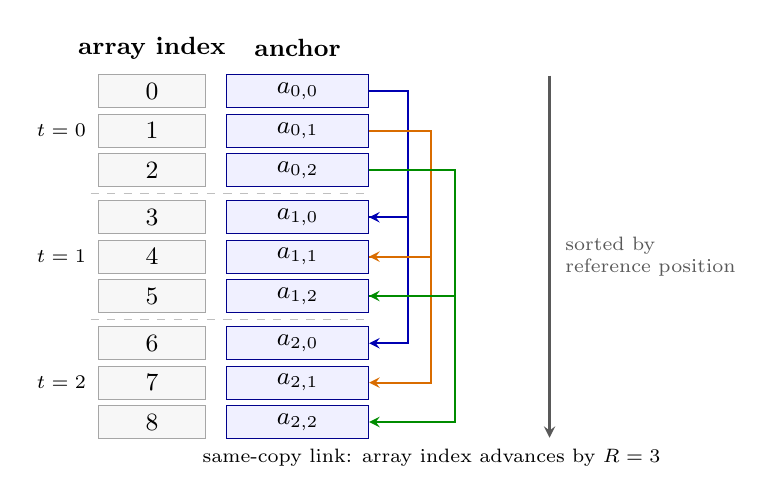
\begin{tikzpicture}[
  index cell/.style={
    draw=black!35,
    fill=black!3,
    minimum width=1.35cm,
    minimum height=0.42cm,
    inner sep=1pt,
    font=\small
  },
  anchor cell/.style={
    draw=blue!55!black,
    fill=blue!6,
    minimum width=1.80cm,
    minimum height=0.42cm,
    inner sep=1pt,
    font=\small
  },
  chain zero/.style={->, >=stealth, line width=0.7pt, blue!70!black},
  chain one/.style={->, >=stealth, line width=0.7pt, orange!85!black},
  chain two/.style={->, >=stealth, line width=0.7pt, green!55!black}
]
  \node[font=\small\bfseries] at (0,0.55) {array index};
  \node[font=\small\bfseries] at (1.85,0.55) {anchor};
  \node[font=\scriptsize] at (-1.15,-0.50) {$t=0$};
  \node[font=\scriptsize] at (-1.15,-2.10) {$t=1$};
  \node[font=\scriptsize] at (-1.15,-3.70) {$t=2$};

  \node[index cell]  (i00) at (0,0.00) {$0$};
  \node[anchor cell] (a00) at (1.85,0.00) {$a_{0,0}$};
  \node[index cell]  (i01) at (0,-0.50) {$1$};
  \node[anchor cell] (a01) at (1.85,-0.50) {$a_{0,1}$};
  \node[index cell]  (i02) at (0,-1.00) {$2$};
  \node[anchor cell] (a02) at (1.85,-1.00) {$a_{0,2}$};

  \draw[black!25,dashed] (-0.78,-1.30) -- (2.78,-1.30);

  \node[index cell]  (i10) at (0,-1.60) {$3$};
  \node[anchor cell] (a10) at (1.85,-1.60) {$a_{1,0}$};
  \node[index cell]  (i11) at (0,-2.10) {$4$};
  \node[anchor cell] (a11) at (1.85,-2.10) {$a_{1,1}$};
  \node[index cell]  (i12) at (0,-2.60) {$5$};
  \node[anchor cell] (a12) at (1.85,-2.60) {$a_{1,2}$};

  \draw[black!25,dashed] (-0.78,-2.90) -- (2.78,-2.90);

  \node[index cell]  (i20) at (0,-3.20) {$6$};
  \node[anchor cell] (a20) at (1.85,-3.20) {$a_{2,0}$};
  \node[index cell]  (i21) at (0,-3.70) {$7$};
  \node[anchor cell] (a21) at (1.85,-3.70) {$a_{2,1}$};
  \node[index cell]  (i22) at (0,-4.20) {$8$};
  \node[anchor cell] (a22) at (1.85,-4.20) {$a_{2,2}$};

  \draw[chain zero] (a00.east) -- (3.25,0.00) -- (3.25,-1.60) -- (a10.east);
  \draw[chain zero] (a10.east) -- (3.25,-1.60) -- (3.25,-3.20) -- (a20.east);
  \draw[chain one]  (a01.east) -- (3.55,-0.50) -- (3.55,-2.10) -- (a11.east);
  \draw[chain one]  (a11.east) -- (3.55,-2.10) -- (3.55,-3.70) -- (a21.east);
  \draw[chain two]  (a02.east) -- (3.85,-1.00) -- (3.85,-2.60) -- (a12.east);
  \draw[chain two]  (a12.east) -- (3.85,-2.60) -- (3.85,-4.20) -- (a22.east);

  \node[font=\scriptsize,align=center] at (3.55,-4.65)
    {same-copy link: array index advances by $R=3$};
  \draw[->,>=stealth,line width=0.8pt,black!65]
    (5.05,0.20) -- (5.05,-4.40)
    node[midway,right=2pt,font=\scriptsize,align=left]
      {sorted by\\reference position};
\end{tikzpicture}
\caption{Coordinate-sorted spaced-copy anchors for the concrete case $R=3$.
As the query contains exact $R$ copies we will have "layers" ($t=0,1,2...$) of the same anchors with the same reference position. Anchor
$a_{t,v}$ is the anchor for $v$-th copy in the query.  Colored arrows follow mark the next anchor in the chain. Naturally each anchor points to the next anchor in the same $v$-th copy. This means that each anchor will just point $R$ anchors forward.}
\label{fig:spaced-copy-anchor-order}
\end{figure}

The construction (d) - minimizer-island comb was created by adjusting gap sizes between query and target islands:
\[
\begin{array}{c|cc}
\text{transition} & \text{target }N\text{-run} & \text{query }N\text{-run}\\
\hline
P\to G & 1475 & 975\\
G\to c_0 & 1250 & 975\\
c_0\to c_1 & 3475 & 3375\\
c_k\to R_k & 475 & 25\ (k\text{ odd}),\ 925\ (k\text{ even})\\
R_k\to c_{k+1} & 1531 & 2081\ (k\text{ odd}),\ 981\ (k\text{ even}).
\end{array}
\]

\info{Default minimap2 parameters}{
As we discussed due to larger shifts between target and query coordinates, the $R_k$ anchors will have larger pentalty due to higher distance from diagonal i.e $\delta$. Minimap2 by default uses max bandwith of $B = \text{bw} = 500$.
Every anchor in $R_k$ and $c_{k+1}$ differ by 550 between the target and query distances, so those anchors fail
the bandwidth check.
This means that the best chain will be going through: $R_{m},c_{m},c_{m-1},...c_0,G,P$ as depicted in the figure~\ref{fig:chaining-runl-inputs}
The original dimentions of constrution can be calculated from the following formula ($r_{k,\ell}$ is the $\ell$-th anchor in $R_k$), $L$ is the count of "islands" in $R_k$:
\resizebox{0.92\linewidth}{!}{%
\(\displaystyle
\begin{aligned}
  B = 500, L = 39,
  s(k) = \begin{cases}
    1 & \text{if } k \text{ is odd} \\
    -1 & \text{if } k \text{ is even} \\
  \end{cases}\\
  c_k \rightarrow c_{k-1}
    &: (3500,\ 3500-100*s(k)),\\
  r_{k,\ell} \rightarrow c_k
    &: (B+(L-1)(\ell-1),\
       B-450*s(k)+(L-1)(\ell-1)),
       &&1\leq\ell\leq L.
\end{aligned}
\)
}
}

\subsubsection{Experiment design}

Minimap2 2.31-r1302 was run with the \texttt{map-ont} preset (default one). 
I added instrumentation to record the score and predecessor arrays.
\begin{itemize}
    \item Let $L\in\{2,4,8,16,32,64\}$ be the number of anchors viewed at the same time similar to our SIMD algorithms. 
    \item Let $\operatorname{Run}_L(j,c) \iff j\geq L-1 \land c\leq n-L \land \bigwedge_{u=0}^{L-1}p_{j-u}=j-u-1$ be the condition used in BioseqDB SIMD algorithms.
    \item Let \(B_L\) be the number of evaluations for which \(\operatorname{Run}_L\) is true
    \item Let \(E_L\) the number of times the first-path loop evaluates \(\operatorname{Run}_L\)
    \item Let \(P_L\) the number that satisfy both bounds \(j\geq L-1\) and \(c\leq n-L\).
    \item Let $q$ be the number of anchors on the first predecessor path.
    \item Let $\operatorname{Fire}_L$ be the observed rate at which my heuristic fires
    \item Let $\operatorname{Contiguous}_L$ be the the ratio $\operatorname{Fire}_L$ but with bounds checks excluded (we measure firing rate but only after bounds checks)
    \item Let $\operatorname{Coverage}_L$ be the fraction of path anchors consumed by vector batches (this is a metric that answers the question "How many anchors we can cover by SIMD batches")
\end{itemize}

The exact definitions are as follows:
\[
  \operatorname{Fire}_L=\frac{B_L}{E_L},
  \qquad
  \operatorname{Contiguous}_L=\frac{B_L}{P_L},
  \qquad
  \operatorname{Coverage}_L=\frac{LB_L}{q}.
\]




\begin{table}[H]
\centering
\caption{Observed first-path branch-firing rate \(100B_L/E_L\), in percent.
The Mosaic, Degraded mosaic, and \(R=1\) Spaced copy rows report medians over three
inputs generated from fixed random-number-generator seeds.  The \(R\geq2\)
Spaced copy row covers the tested powers of two from 2 through 64, all of
which gave zero.  Minimizer-island-comb values are deterministic and agreed
with the recorded counters.}
\label{tab:chaining-runl-firing}
\scriptsize
\setlength{\tabcolsep}{3.2pt}
\begin{tabular}{lrrrrrr}
\toprule
Input & \(L=2\) & \(L=4\) & \(L=8\) & \(L=16\) & \(L=32\) & \(L=64\) \\
\midrule
(a) Mosaic                     &   1.17 &  0.59 &  0.29 &  0.14 &  0.07 &  0.02 \\
(b) Degraded mosaic (independent \(A'\)) & 100.00 & 99.94 & 99.74 & 99.24 & 97.01 & 91.12 \\
(c) Spaced copy, \(R=1\)       & 100.00 & 98.97 & 94.12 & 88.89 & 80.00 & 66.67 \\
(c) Spaced copy, \(R\geq2\)   &   0.00 &  0.00 &  0.00 &  0.00 &  0.00 &  0.00 \\
(d) Minimizer-island comb, \(m=2\)    & 95.74 & 84.62 & 45.45 & 29.41 & 6.67 & 0.00 \\
(d) Minimizer-island comb, \(m=1024\) &  4.21 &  2.10 &  0.96 &  0.48 & 0.19 & 0.00 \\
\bottomrule
\end{tabular}
\end{table}

We can make the following observations:
\begin{itemize}
  \item For minimizer-island the prefix will contain some $C > 0$ anchors, meaning that we will get only continuous parts in $R_m$ at the end and in the sequence prefix: $B_L \simeq \left\lfloor\frac{39}{L}\right\rfloor + \left\lfloor\frac{C}{L}\right\rfloor, q = m + C$
  This means that for $L = const:$ $\operatorname{Fire}_L, \operatorname{Coverage}_L < \theta(1/m)$ and for large enough $L > 39 \land m \rightarrow \infty$ they will approach $0$.
  \item For spaced copy the anchors are always separated by $R$ so $\operatorname{Fire}_L$ should be zero for all $R > 0$
  \item Degraded mosaic is just simulating two random fragments, so $\operatorname{Fire}_L$ should be almost $100\%$ with high measured divergence.
  \item Mosaic in this case was simulated with zero divergence, so the $\operatorname{Fire}_L$ should measure anchors only in the fillers between equal parts i.e $0\% < \operatorname{Fire}_L < \frac{|U_i|*3}{|U_i|*3+|A|} < 4\%$
\end{itemize}

The table~\ref{tab:chaining-runl-firing} confirms our assumptions.

Now we would like to see how divergence $\delta$ affects the mosaic rates.
Table~\ref{tab:chaining-runl-mosaic-divergence} shows selected data points
from Mosaic runs at \(\delta\). $s_{\delta}$ is the number of substitutions made to the target sequence. We can see that the higher number of same-target anchor alternatives (multiple query positions per anchor), the worse results we get (as predicted).

% Generated by runl_dense_divergence_audit.py. Do not edit by hand.

% manifest sha256: ba60e4b6e82dd32547c854f6c3d90273050a519a777c327c2cce4d1829c8fbca

% runner aggregate sha256: ed840411aee062d90a0b6cab2f98b13cf1acd5cd2e2e46911f8f46fd2ebde386

\def\RunLDenseGroupedMedianCoordinates{%
  (0,97.68786127) (0.25024414,93.50982752) (0.50048828,89.55342903) (0.75073242,85.89075158)%
  (1.00097656,82.23867526) (1.2512207,78.86191931) (1.50146484,75.55307974) (1.74865723,72.23425592)%
  (1.99890137,69.33440257) (2.24914551,66.26081384) (2.49938965,63.27348509) (2.74963379,60.77755511)%
  (2.99987793,58.44486934) (3.25012207,55.95664993) (3.50036621,53.5011551) (3.75061035,51.25976012)%
  (4.00085449,49.20379604) (4.25109863,47.00779179) (4.50134277,45.13295536) (4.74853516,43.1629393)%
  (4.9987793,41.4114621) (5.24902344,39.71540491) (5.49926758,38.11897106) (5.74951172,36.41321784)%
  (5.99975586,34.78051134) (6.25,33.48081409) (6.50024414,32.36381167) (6.75048828,31.08824948)%
  (7.00073242,29.6522859) (7.25097656,28.57602833) (7.5012207,27.22664736) (7.75146484,26.01769912)%
  (7.99865723,25.08043758) (8.24890137,24.08301158) (8.49914551,23.03547012) (8.74938965,21.84508968)%
  (8.99963379,21.01029601) (9.24987793,19.99517801) (9.50012207,19.16438135) (9.75036621,18.34124367)%
  (10.00061035,17.23111576) (10.25085449,16.6091077) (10.50109863,15.78143833) (10.75134277,15.31661845)%
  (10.99853516,14.6142136) (11.2487793,14.02409639) (11.49902344,13.47826087) (11.74926758,13.05781137)%
  (11.99951172,12.32326478) (12.24975586,11.81482077) (12.5,11.26760563) (12.75024414,10.72463768)%
  (13.00048828,10.19569944) (13.25073242,9.724343) (13.50097656,9.28175018) (13.7512207,8.81808673)%
  (14.00146484,8.51303508) (14.24865723,8.22622108) (14.49890137,7.71890327) (14.74914551,7.50221364)%
  (14.99938965,7.17676402) (15.24963379,6.80666184) (15.49987793,6.68971617) (15.75012207,6.40592306)%
  (16.00036621,6.20130131) (16.25061035,5.95028067) (16.50085449,5.64057367) (16.75109863,5.38547844)%
  (17.00134277,5.0669446) (17.24853516,4.79743281) (17.4987793,4.57023733) (17.74902344,4.36702256)%
  (17.99926758,4.22795595) (18.24951172,4.17637138) (18.49975586,4.0138075) (18.75,3.8060061)%
  (19.00024414,3.6009967) (19.25048828,3.45492528) (19.50073242,3.33921978) (19.75097656,3.16313423)%
  (20.0012207,3.03516942)%
}

\def\RunLDenseGroupedMinimumCoordinates{%
  (0,97.63691522) (0.25024414,93.40420391) (0.50048828,89.4715676) (0.75073242,85.67526312)%
  (1.00097656,82.18782581) (1.2512207,78.82730924) (1.50146484,75.14868992) (1.74865723,71.86522262)%
  (1.99890137,68.93344026) (2.24914551,66.12127045) (2.49938965,62.95702373) (2.74963379,60.29458854)%
  (2.99987793,57.76103854) (3.25012207,55.45585643) (3.50036621,53.03078897) (3.75061035,50.91375441)%
  (4.00085449,48.60442733) (4.25109863,46.78362573) (4.50134277,45.01241888) (4.74853516,43.13316764)%
  (4.9987793,41.33354653) (5.24902344,39.45632942) (5.49926758,37.8170761) (5.74951172,36.07868223)%
  (5.99975586,34.19664269) (6.25,32.78714731) (6.50024414,31.49568552) (6.75048828,30.37469042)%
  (7.00073242,29.09352059) (7.25097656,27.77644519) (7.5012207,26.54838967) (7.75146484,25.39987204)%
  (7.99865723,24.44053708) (8.24890137,23.2238472) (8.49914551,22.23644217) (8.74938965,20.96748358)%
  (8.99963379,20.18730489) (9.24987793,19.42152071) (9.50012207,18.64637565) (9.75036621,17.81019558)%
  (10.00061035,16.81373335) (10.25085449,16.33667335) (10.50109863,15.7359186) (10.75134277,15.19859065)%
  (10.99853516,14.49228792) (11.2487793,13.86709367) (11.49902344,13.30664532) (11.74926758,12.38796415)%
  (11.99951172,11.66026871) (12.24975586,11.19104716) (12.5,10.6314948) (12.75024414,10.19413598)%
  (13.00048828,9.86231188) (13.25073242,9.32169456) (13.50097656,8.90454837) (13.7512207,8.5563211)%
  (14.00146484,8.27531012) (14.24865723,7.84627702) (14.49890137,7.54626292) (14.74914551,7.04958744)%
  (14.99938965,6.85512933) (15.24963379,6.67573841) (15.49987793,6.4061499) (15.75012207,6.10283518)%
  (16.00036621,5.78108736) (16.25061035,5.44130591) (16.50085449,5.15076382) (16.75109863,4.87452898)%
  (17.00134277,4.66832438) (17.24853516,4.44194997) (17.4987793,4.32553669) (17.74902344,4.10289286)%
  (17.99926758,3.82522407) (18.24951172,3.70044053) (18.49975586,3.59913621) (18.75,3.37762126)%
  (19.00024414,3.26008789) (19.25048828,3.0499002) (19.50073242,2.92285577) (19.75097656,2.82161645)%
  (20.0012207,2.66093053)%
}

\def\RunLDenseGroupedMaximumCoordinates{%
  (0,97.68865265) (0.25024414,93.5249501) (0.50048828,89.67617826) (0.75073242,85.90101219)%
  (1.00097656,82.29057907) (1.2512207,78.93396977) (1.50146484,75.58549888) (1.74865723,72.65045835)%
  (1.99890137,69.42451777) (2.24914551,66.83144634) (2.49938965,64.08417025) (2.74963379,61.17572089)%
  (2.99987793,58.44770848) (3.25012207,56.19980726) (3.50036621,53.60907701) (3.75061035,51.3351933)%
  (4.00085449,49.44107314) (4.25109863,47.55289421) (4.50134277,45.3399695) (4.74853516,43.44334698)%
  (4.9987793,41.62859662) (5.24902344,39.99039462) (5.49926758,38.24496671) (5.74951172,36.65005626)%
  (5.99975586,35.3648757) (6.25,34.15924946) (6.50024414,32.8099968) (6.75048828,31.49883842)%
  (7.00073242,30.30691562) (7.25097656,28.81641157) (7.5012207,27.73945131) (7.75146484,26.81008188)%
  (7.99865723,25.99179207) (8.24890137,24.6879781) (8.49914551,23.56451613) (8.74938965,22.51410153)%
  (8.99963379,21.22409483) (9.24987793,20.11128135) (9.50012207,19.19549477) (9.75036621,18.3446273)%
  (10.00061035,17.63756656) (10.25085449,16.83870968) (10.50109863,15.97160603) (10.75134277,15.38958417)%
  (10.99853516,14.80406386) (11.2487793,14.2408377) (11.49902344,13.81589553) (11.74926758,13.38272003)%
  (11.99951172,12.89078197) (12.24975586,12.19473008) (12.5,11.83089535) (12.75024414,11.43361129)%
  (13.00048828,10.77700265) (13.25073242,10.29176018) (13.50097656,9.7169887) (13.7512207,9.46432861)%
  (14.00146484,9.00280336) (14.24865723,8.60714858) (14.49890137,8.28383368) (14.74914551,7.82741198)%
  (14.99938965,7.57442028) (15.24963379,7.27301919) (15.49987793,7.0195165) (15.75012207,6.6083888)%
  (16.00036621,6.27953544) (16.25061035,6.07663941) (16.50085449,5.6936648) (16.75109863,5.42188001)%
  (17.00134277,5.21125631) (17.24853516,4.82333146) (17.4987793,4.79013137) (17.74902344,4.61464509)%
  (17.99926758,4.47330447) (18.24951172,4.29659319) (18.49975586,4.15097364) (18.75,3.90806439)%
  (19.00024414,3.69688725) (19.25048828,3.59884837) (19.50073242,3.49302996) (19.75097656,3.47561464)%
  (20.0012207,3.36161357)%
}

\def\RunLDenseFireFourMedianCoordinates{%
  (0,0.58823529) (0.25024414,1.06277805) (0.50048828,1.5610652) (0.75073242,1.99795953)%
  (1.00097656,2.61177895) (1.2512207,3.19739276) (1.50146484,3.88271879) (1.74865723,4.4653349)%
  (1.99890137,5.14306744) (2.24914551,5.78218563) (2.49938965,6.65384615) (2.74963379,7.44263581)%
  (2.99987793,8.16346922) (3.25012207,8.87826706) (3.50036621,9.82496353) (3.75061035,10.61233153)%
  (4.00085449,11.46903038) (4.25109863,12.26238875) (4.50134277,13.05845743) (4.74853516,14.01020987)%
  (4.9987793,14.96756256) (5.24902344,16.17295748) (5.49926758,17.16571706) (5.74951172,18.29102167)%
  (5.99975586,19.33434959) (6.25,20.31330917) (6.50024414,21.13970588) (6.75048828,22.22371065)%
  (7.00073242,23.51407001) (7.25097656,24.46957007) (7.5012207,25.50774038) (7.75146484,26.7323862)%
  (7.99865723,27.86885246) (8.24890137,29.08570568) (8.49914551,30.25932177) (8.74938965,31.57400157)%
  (8.99963379,32.6959847) (9.24987793,33.95734983) (9.50012207,35.17904509) (9.75036621,36.44039176)%
  (10.00061035,37.98623064) (10.25085449,39.27571728) (10.50109863,40.49689441) (10.75134277,41.60464694)%
  (10.99853516,42.75722437) (11.2487793,43.88878522) (11.49902344,45.01705191) (11.74926758,45.94025278)%
  (11.99951172,46.876813) (12.24975586,48.01019408) (12.5,48.7433208) (12.75024414,49.69915764)%
  (13.00048828,51.15853659) (13.25073242,52.09531635) (13.50097656,53.36820084) (13.7512207,54.74064626)%
  (14.00146484,55.83886865) (14.24865723,57.0280252) (14.49890137,58.23594267) (14.74914551,59.87889661)%
  (14.99938965,60.48460145) (15.24963379,62.17150761) (15.49987793,62.98791822) (15.75012207,63.62359551)%
  (16.00036621,64.37485284) (16.25061035,65.24419156) (16.50085449,66.62662182) (16.75109863,67.49150898)%
  (17.00134277,69.3504569) (17.24853516,70.48975512) (17.4987793,71.06981416) (17.74902344,71.57655382)%
  (17.99926758,72.51148545) (18.24951172,73.05819021) (18.49975586,74.18436044) (18.75,75.25503531)%
  (19.00024414,75.77265584) (19.25048828,76.44879598) (19.50073242,76.99256111) (19.75097656,78.0101904)%
  (20.0012207,79.4133623)%
}

\def\RunLDenseFireFourMinimumCoordinates{%
  (0,0.58177647) (0.25024414,1.0083478) (0.50048828,1.47304988) (0.75073242,1.98446208)%
  (1.00097656,2.57267816) (1.2512207,3.19037657) (1.50146484,3.81693037) (1.74865723,4.37426264)%
  (1.99890137,5.0831793) (2.24914551,5.78061848) (2.49938965,6.58648339) (2.74963379,7.4092104)%
  (2.99987793,8.1622533) (3.25012207,8.80427118) (3.50036621,9.67112025) (3.75061035,10.40794979)%
  (4.00085449,11.24399359) (4.25109863,12.04216933) (4.50134277,13.01484541) (4.74853516,14.0038773)%
  (4.9987793,14.96622409) (5.24902344,16.02935954) (5.49926758,17.08206687) (5.74951172,17.97599901)%
  (5.99975586,19.11671924) (6.25,20.04365691) (6.50024414,21.03475307) (6.75048828,21.96969697)%
  (7.00073242,22.96968056) (7.25097656,24.32769615) (7.5012207,25.2007325) (7.75146484,25.90584879)%
  (7.99865723,26.82253848) (8.24890137,28.22304833) (8.49914551,29.42605527) (8.74938965,30.84083152)%
  (8.99963379,32.19720989) (9.24987793,33.85711971) (9.50012207,34.85845951) (9.75036621,36.26133692)%
  (10.00061035,37.63958083) (10.25085449,38.94037419) (10.50109863,40.44104571) (10.75134277,41.12367618)%
  (10.99853516,42.73143905) (11.2487793,43.39064522) (11.49902344,44.36936937) (11.74926758,45.153351)%
  (11.99951172,46.6461064) (12.24975586,47.49561489) (12.5,48.51778656) (12.75024414,49.53159259)%
  (13.00048828,50.84401058) (13.25073242,52.02716608) (13.50097656,53.30277141) (13.7512207,54.10628019)%
  (14.00146484,55.66058002) (14.24865723,56.92843159) (14.49890137,58.20269375) (14.74914551,59.36870383)%
  (14.99938965,60.40162455) (15.24963379,61.38229927) (15.49987793,61.79234472) (15.75012207,63.05658627)%
  (16.00036621,64.24384525) (16.25061035,65.02602934) (16.50085449,66.22754491) (16.75109863,67.18221363)%
  (17.00134277,68.29626008) (17.24853516,69.97765086) (17.4987793,70.15667744) (17.74902344,71.20603015)%
  (17.99926758,71.66666667) (18.24951172,72.44975833) (18.49975586,73.43429158) (18.75,74.86353002)%
  (19.00024414,75.42617362) (19.25048828,76.06299213) (19.50073242,76.41783171) (19.75097656,76.92715232)%
  (20.0012207,77.57656458)%
}

\def\RunLDenseFireFourMaximumCoordinates{%
  (0,0.59315837) (0.25024414,1.1842215) (0.50048828,1.78813559) (0.75073242,2.29263266)%
  (1.00097656,2.80365694) (1.2512207,3.31125828) (1.50146484,3.97625045) (1.74865723,4.71611722)%
  (1.99890137,5.29739777) (2.24914551,6.01154975) (2.49938965,6.78374988) (2.74963379,7.57441792)%
  (2.99987793,8.47236181) (3.25012207,9.27898402) (3.50036621,10.17161992) (3.75061035,11.07314469)%
  (4.00085449,11.95379754) (4.25109863,12.66998342) (4.50134277,13.54366197) (4.74853516,14.5605345)%
  (4.9987793,15.37830874) (5.24902344,16.44949193) (5.49926758,17.33934886) (5.74951172,18.37750404)%
  (5.99975586,19.35809957) (6.25,20.35272915) (6.50024414,21.65546329) (6.75048828,22.58107746)%
  (7.00073242,23.98463227) (7.25097656,25.45121263) (7.5012207,26.49168101) (7.75146484,27.57562473)%
  (7.99865723,28.76712329) (8.24890137,30.09428224) (8.49914551,31.38686131) (8.74938965,32.88782816)%
  (8.99963379,34.13804277) (9.24987793,35.10445797) (9.50012207,36.24811904) (9.75036621,37.40432046)%
  (10.00061035,38.72030518) (10.25085449,39.53040126) (10.50109863,40.55068836) (10.75134277,41.80505415)%
  (10.99853516,43.18558028) (11.2487793,44.44236877) (11.49902344,45.86265931) (11.74926758,47.79898714)%
  (11.99951172,49.3158834) (12.24975586,50.55320861) (12.5,52.09997951) (12.75024414,53.30149502)%
  (13.00048828,54.18242959) (13.25073242,55.35904539) (13.50097656,56.72868888) (13.7512207,57.68978342)%
  (14.00146484,58.36635843) (14.24865723,60.09874327) (14.49890137,61.02040816) (14.74914551,62.71929825)%
  (14.99938965,63.26293804) (15.24963379,63.91872957) (15.49987793,64.95867769) (15.75012207,65.83273767)%
  (16.00036621,67.29514141) (16.25061035,68.4171959) (16.50085449,69.52122409) (16.75109863,70.27161724)%
  (17.00134277,70.76653307) (17.24853516,71.94226386) (17.4987793,72.60692464) (17.74902344,73.84694666)%
  (17.99926758,75.70680628) (18.24951172,76.531151) (18.49975586,76.95157449) (18.75,77.6652452)%
  (19.00024414,78.3877879) (19.25048828,79.71838614) (19.50073242,80.33769063) (19.75097656,80.92896175)%
  (20.0012207,81.92837466)%
}

\def\RunLDenseCoverageFourMedianCoordinates{%
  (0,2.31213873) (0.25024414,4.11976048) (0.50048828,5.96491228) (0.75073242,7.53990535)%
  (1.00097656,9.68802631) (1.2512207,11.67014949) (1.50146484,13.91055228) (1.74865723,15.75129534)%
  (1.99890137,17.82241352) (2.24914551,19.70977516) (2.49938965,22.18659827) (2.74963379,24.33667335)%
  (2.99987793,26.23003451) (3.25012207,28.04368776) (3.50036621,30.35326306) (3.75061035,32.19834179)%
  (4.00085449,34.13221811) (4.25109863,35.85830187) (4.50134277,37.53094306) (4.74853516,39.45686901)%
  (4.9987793,41.31755676) (5.24902344,43.55798617) (5.49926758,45.32287749) (5.74951172,47.24132416)%
  (5.99975586,48.94677601) (6.25,50.48668651) (6.50024414,51.74353206) (6.75048828,53.33547661)%
  (7.00073242,55.15132003) (7.25097656,56.44369315) (7.5012207,57.80030574) (7.75146484,59.34030571)%
  (7.99865723,60.71428571) (8.24890137,62.12998713) (8.49914551,63.44406016) (8.74938965,64.85964771)%
  (8.99963379,66.02316602) (9.24987793,67.28489638) (9.50012207,68.46265527) (9.75036621,69.63536625)%
  (10.00061035,71.01600837) (10.25085449,72.12272107) (10.50109863,73.13516545) (10.75134277,74.02503028)%
  (10.99853516,74.92339945) (11.2487793,75.77929923) (11.49902344,76.60809286) (11.74926758,77.26870118)%
  (11.99951172,77.92333039) (12.24975586,78.69537275) (12.5,79.18341103) (12.75024414,79.80676329)%
  (13.00048828,80.73129661) (13.25073242,81.30811157) (13.50097656,82.07190541) (13.7512207,82.87070561)%
  (14.00146484,83.49219063) (14.24865723,84.14810066) (14.49890137,84.79691764) (14.74914551,85.652418)%
  (14.99938965,85.96025424) (15.24963379,86.797007) (15.49987793,87.19144488) (15.75012207,87.49396427)%
  (16.00036621,87.84641337) (16.25061035,88.24755491) (16.50085449,88.87108405) (16.75109863,89.25248637)%
  (17.00134277,90.0505091) (17.24853516,90.52547132) (17.4987793,90.76330981) (17.74902344,90.96893313)%
  (17.99926758,91.34313962) (18.24951172,91.55891093) (18.49975586,91.99646785) (18.75,92.40404689)%
  (19.00024414,92.59822357) (19.25048828,92.84910815) (19.50073242,93.04864344) (19.75097656,93.41682723)%
  (20.0012207,93.91360206)%
}

\def\RunLDenseCoverageFourMinimumCoordinates{%
  (0,2.28718692) (0.25024414,3.91496189) (0.50048828,5.64283424) (0.75073242,7.49183072)%
  (1.00097656,9.55337951) (1.2512207,11.64677804) (1.50146484,13.69906962) (1.74865723,15.46730846)%
  (1.99890137,17.64234162) (2.24914551,19.70522269) (2.49938965,21.99904352) (2.74963379,24.24725187)%
  (2.99987793,26.22689611) (3.25012207,27.85879353) (3.50036621,29.98486418) (3.75061035,31.72578717)%
  (4.00085449,33.63142766) (4.25109863,35.38522954) (4.50134277,37.44079634) (4.74853516,39.44431061)%
  (4.9987793,41.31500683) (5.24902344,43.29682629) (5.49926758,45.17684887) (5.74951172,46.71274715)%
  (5.99975586,48.59663192) (6.25,50.06815813) (6.50024414,51.58603012) (6.75048828,52.96803653)%
  (7.00073242,54.39538425) (7.25097656,56.25450757) (7.5012207,57.40413926) (7.75146484,58.30791459)%
  (7.99865723,59.45119498) (8.24890137,61.13213624) (8.49914551,62.51612903) (8.74938965,64.07735697)%
  (8.99963379,65.5108459) (9.24987793,67.18636985) (9.50012207,68.15768302) (9.75036621,69.47148258)%
  (10.00061035,70.71163466) (10.25085449,71.83870968) (10.50109863,73.08959421) (10.75134277,73.64191578)%
  (10.99853516,74.90359897) (11.2487793,75.40562249) (11.49902344,76.1352657) (11.74926758,76.70660127)%
  (11.99951172,77.76349614) (12.24975586,78.34753255) (12.5,79.03420523) (12.75024414,79.6985247)%
  (13.00048828,80.53475074) (13.25073242,81.26657558) (13.50097656,82.03319169) (13.7512207,82.50460405)%
  (14.00146484,83.39233988) (14.24865723,84.09383033) (14.49890137,84.77928761) (14.74914551,85.39000241)%
  (14.99938965,85.91831822) (15.24963379,86.40924781) (15.49987793,86.61151715) (15.75012207,87.2243163)%
  (16.00036621,87.78534241) (16.25061035,88.14755413) (16.50085449,88.69286287) (16.75109863,89.11684565)%
  (17.00134277,89.60153932) (17.24853516,90.31327618) (17.4987793,90.38769625) (17.74902344,90.81877904)%
  (17.99926758,91.00529101) (18.24951172,91.31863727) (18.49975586,91.70606619) (18.75,92.25594618)%
  (19.00024414,92.46845109) (19.25048828,92.70633397) (19.50073242,92.83768627) (19.75097656,93.02474574)%
  (20.0012207,93.26076517)%
}

\def\RunLDenseCoverageFourMaximumCoordinates{%
  (0,2.33115121) (0.25024414,4.57437384) (0.50048828,6.78838575) (0.75073242,8.58038081)%
  (1.00097656,10.34455064) (1.2512207,12.04819277) (1.50146484,14.20993409) (1.74865723,16.52627357)%
  (1.99890137,18.28388132) (2.24914551,20.37215271) (2.49938965,22.54650417) (2.74963379,24.68780019)%
  (2.99987793,27.02139595) (3.25012207,29.03380868) (3.50036621,31.17382938) (3.75061035,33.24783584)%
  (4.00085449,35.19409689) (4.25109863,36.72194184) (4.50134277,38.52255428) (4.74853516,40.5355568)%
  (4.9987793,42.09345195) (5.24902344,44.05667174) (5.49926758,45.62444854) (5.74951172,47.38530638)%
  (5.99975586,48.98481215) (6.25,50.54751818) (6.50024414,52.50878875) (6.75048828,53.84676839)%
  (7.00073242,55.79316949) (7.25097656,57.7276725) (7.5012207,59.0425957) (7.75146484,60.3646833)%
  (7.99865723,61.76470588) (8.24890137,63.2622073) (8.49914551,64.66165414) (8.74938965,66.21816434)%
  (8.99963379,67.4617786) (9.24987793,68.39195577) (9.50012207,69.45935122) (9.75036621,70.50336646)%
  (10.00061035,71.65089042) (10.25085449,72.33667335) (10.50109863,73.17899492) (10.75134277,74.18321589)%
  (10.99853516,75.25038058) (11.2487793,76.18895116) (11.49902344,77.21377102) (11.74926758,78.553137)%
  (11.99951172,79.55854127) (12.24975586,80.35171863) (12.5,81.31095124) (12.75024414,82.03243589)%
  (13.00048828,82.54883125) (13.25073242,83.22255145) (13.50097656,83.98462524) (13.7512207,84.50568819)%
  (14.00146484,84.86594638) (14.24865723,85.76461169) (14.49890137,86.22927181) (14.74914551,87.06240487)%
  (14.99938965,87.32281573) (15.24963379,87.63307452) (15.49987793,88.11659193) (15.75012207,88.51513695)%
  (16.00036621,89.16646649) (16.25061035,89.65351684) (16.50085449,90.12237063) (16.75109863,90.43534034)%
  (17.00134277,90.63928772) (17.24853516,91.11610006) (17.4987793,91.38096764) (17.74902344,91.86633544)%
  (17.99926758,92.57362356) (18.24951172,92.87945535) (18.49975586,93.03367192) (18.75,93.29278053)%
  (19.00024414,93.55173791) (19.25048828,94.01996008) (19.50073242,94.2341479) (19.75097656,94.43647378)%
  (20.0012207,94.77374124)%
}

\def\RunLDenseSelectedTableRows{%
  \(\delta=0\) & 0 & 0.000 & 97.69 [97.64, 97.69] & 0.59 [0.58, 0.59] & 2.31 [2.29, 2.33] \\%
  \(\delta=0.0025\) & 82 & 0.250 & 93.51 [93.40, 93.52] & 1.06 [1.01, 1.18] & 4.12 [3.91, 4.57] \\%
  \(\delta=0.0050\) & 164 & 0.500 & 89.55 [89.47, 89.68] & 1.56 [1.47, 1.79] & 5.96 [5.64, 6.79] \\%
  \(\delta=0.0100\) & 328 & 1.001 & 82.24 [82.19, 82.29] & 2.61 [2.57, 2.80] & 9.69 [9.55, 10.34] \\%
  \(\delta=0.0200\) & 655 & 1.999 & 69.33 [68.93, 69.42] & 5.14 [5.08, 5.30] & 17.82 [17.64, 18.28] \\%
  \(\delta=0.0500\) & 1638 & 4.999 & 41.41 [41.33, 41.63] & 14.97 [14.97, 15.38] & 41.32 [41.32, 42.09] \\%
  \(\delta=0.1000\) & 3277 & 10.001 & 17.23 [16.81, 17.64] & 37.99 [37.64, 38.72] & 71.02 [70.71, 71.65] \\%
  \(\delta=0.2000\) & 6554 & 20.001 & 3.04 [2.66, 3.36] & 79.41 [77.58, 81.93] & 93.91 [93.26, 94.77] \\%
}

\def\RunLDenseIndependentTableRow{%
  Independent \(A'\) & \text{n/a} & 75.043 & 0.00 [0.00, 0.00] & 99.94 [99.90, 100.00] & 99.98 [99.98, 100.00] \\%
}


\begin{table}[H]
\centering
\caption{Few most important data points for mosaic construction for different values of
\(\delta\) and degraded mosaic (should have effective high divergence).  Each
entry in the last three columns id the median followed by the observed
minimum and maximum over three inputs generated from fixed
random-number-generator seeds, in percent.}
\label{tab:chaining-runl-mosaic-divergence}
\scriptsize
\setlength{\tabcolsep}{3.0pt}
\begin{tabular}{lrrlll}
\toprule
Case & \(s_{\delta}\) & \(100\widehat{\delta}\) &
\shortstack{Path anchors with\\same-target alternatives} &
\(100\operatorname{Fire}_4\) &
\(100\operatorname{Coverage}_4\) \\
& & (\%) & (\%) & (\%) & (\%) \\
\midrule
\RunLDenseSelectedTableRows
\midrule
\RunLDenseIndependentTableRow
\bottomrule
\end{tabular}
\end{table}

Let's consider that we are looking at mosaic with divergence rate $\delta = 0$, so $A = A'$. Then we have $h$ pairwise-disjoint "blocking" minimizer windows $W_1, \ldots, W_h$. Each $W_i$ has some minimizer that now forms an anchor that makes $Run_L(j,c)$ evaluation false. $W_i$ covers $k+w-1$ bases. Each of the windows needs to receive at least one subsitution 
so they're changed and do not generate one anchor with two different positions.
So with probability $\frac{(s_{\delta})_h}{(M)_h}$ all $h$ windows will receive at least one substitution (for $(x)_h = x(x-1)\cdots(x-h+1)$).
We can choose one base from every window with $b^h$ ways, so this gives us very loose upper bound on the probability:
\[
\begin{aligned}
  \Pr_{\pi}\!\left[
    \operatorname{Run}_L(j,c)\text{ changes from false to true}
  \right]
  &\leq
  \Pr_{\pi}\!\left[
    S_{\delta}\cap W_i\neq\varnothing
    \text{ for every }i
  \right] \\
  &\leq
  b^h\frac{(s_{\delta})_h}{(M)_h}
  \leq
  (b\widehat{\delta})^h .
\end{aligned}
\]
Obiously disjoint-window model is a bad assumption as substitution can affect several overlapping windows and conversely with high divergence we can spontaneusly get random matches with other fragments like $U_i$ (although this is unlikely).
However we can loosely bound the probability by $\theta((k\widehat{\delta})^h)$. This gives us idea that the worst sequences are the one with perfect repeats (low divergence).

Figure~\ref{fig:chaining-runl-mosaic-divergence} shows the results for mosaic for different levels of divergence (the degraded mosaic - as control sample - is show separately as a gray rectangle on the right side of chart)

\begin{figure}[H]
\centering
\begin{tikzpicture}[
  font=\scriptsize,
  mosaic grouped/.style={
    draw=chainBlue!90!black,line width=.85pt},
  mosaic grouped range/.style={
    draw=chainBlue!45,line width=.35pt},
  mosaic fire/.style={
    draw=chainOrange!95!black,line width=.85pt,dashed},
  mosaic fire range/.style={
    draw=chainOrange!55,line width=.35pt,densely dashed}
]
\begin{scope}[x=.48cm,y=.045cm]
  \path[fill=black!3,draw=black!20]
    (21.2,0) rectangle (23.2,100);

  \foreach \yy in {0,25,50,75,100} {
    \draw[black!12] (0,\yy)--(20.5,\yy);
    \node[anchor=east] at (-.25,\yy) {\yy};
  }

  \draw[mosaic grouped range]
    plot coordinates {\RunLDenseGroupedMinimumCoordinates};
  \draw[mosaic grouped range]
    plot coordinates {\RunLDenseGroupedMaximumCoordinates};
  \draw[mosaic fire range]
    plot coordinates {\RunLDenseFireFourMinimumCoordinates};
  \draw[mosaic fire range]
    plot coordinates {\RunLDenseFireFourMaximumCoordinates};

  \draw[mosaic grouped]
    plot[mark=*,mark size=.42pt]
    coordinates {\RunLDenseGroupedMedianCoordinates};
  \draw[mosaic fire]
    plot[mark=x,mark size=.42pt]
    coordinates {\RunLDenseFireFourMedianCoordinates};

  \draw[->] (0,0)--(0,105);
  \draw[->] (0,0)--(20.8,0);
  \foreach \xx in {0,5,10,15,20} {
    \draw (\xx,-2)--(\xx,2);
    \node[anchor=north] at (\xx,-4.5) {\xx};
  }

  \node[rotate=90] at (-1.55,50) {reported value (\%)};
  \node at (10,-13)
    {realized internal divergence \(100\widehat{\delta}\) (\%)};

  \node[circle,draw=chainBlue!90!black,fill=white,
        minimum size=3.1pt,inner sep=0pt]
    at (22.2,0) {};
  \node[rectangle,draw=chainOrange!95!black,fill=white,
        minimum size=3.1pt,inner sep=0pt]
    at (22.2,99.94) {};
  \node[rotate=90,text=black!58] at (22.2,50)
    {independent \(A'\) control};
  \node[anchor=north,align=center] at (22.2,-4.5)
    {75.043\\outside axis};

  \draw[mosaic grouped] (.4,110)--(1.4,110);
  \node[anchor=west,align=left] at (1.65,110)
    {path anchors with\\same-target alternatives};
  \draw[mosaic fire] (12.0,110)--(13.0,110);
  \node[anchor=west] at (13.25,110) {\(\operatorname{Fire}_4\)};
\end{scope}
\end{tikzpicture}
\caption{The lighter colours represent minimum/maximum while the darker ones represent median. As we can see the chart confirms that the $Run_L$ firing rates are tied to number of anchors with same-target positions which are competing for the same anchor. Additionally we observe that divergence levels of at least 12\% mitigate the negative effect of highly-repetive query.}
\label{fig:chaining-runl-mosaic-divergence}
\end{figure}

As we can see from Figure~\ref{fig:chaining-runl-mosaic-divergence}, table~\ref{tab:chaining-runl-mosaic-divergence} and table~\ref{tab:chaining-runl-firing} the most inconvenient case is the high number of repetitions in the query. These repetitions can be mitigated by increased divergence levels. This was intuitive consulsion that we now sucessfully confirmed with the experiments.

\subsubsection{Random-sequence subsitutions}

I also wanted to measure effects of random sequences (not specially constructed) on the $Run_L$ firing rates:
\begin{itemize}
  \item We generate random sequences query/target parameterized by their lengths: $|T|$ and $|Q|$. We choose $N$ positions in target to be the query and replace its fragments accordingly. By default we test each such occurence base with probability $0.001$ to be substituted, $0.0005$ to be inserted/deleted.
  \item Here I also use the default minimap2 parameters: $k=15$, $w=10$, occurrence filtering, and chaining scores.
\end{itemize}

\begin{figure}[H]
\centering
\begin{tikzpicture}[
  font=\scriptsize,
  runl four/.style={draw=chainBlue!90!black,line width=.85pt},
  runl eight/.style={
    draw=chainOrange!95!black,line width=.85pt,dashed},
  runl sixteen/.style={
    draw=chainGreen!70!black,line width=.9pt,densely dotted},
  runl mark four/.style={
    circle,draw=chainBlue!90!black,fill=white,
    minimum size=4.4pt,inner sep=0pt},
  runl mark eight/.style={
    rectangle,draw=chainOrange!95!black,fill=white,
    minimum size=4.4pt,inner sep=0pt},
  runl mark sixteen/.style={
    circle,draw=chainGreen!70!black,fill=chainGreen!55,
    minimum size=4.4pt,inner sep=0pt}
]
  % Panel (b): corrected ten-input compact series.
  \begin{scope}[x=1cm,y=.038cm,xshift=1.55cm,yshift=.70cm]
    \node[anchor=west,font=\bfseries\footnotesize] at (-1.25,112)
      {(b) Ten-input compact series: \(\lvert T\rvert=4.5\,\mathrm{Mb}\),
       \(\lvert Q\rvert=997\) to \(1002\,\mathrm{bp}\)};

    \path[fill=chainBlue!45,fill opacity=.15]
      (.20,93.1008) rectangle (11.7051,95.7639);
    \path[fill=chainOrange!55,fill opacity=.13]
      (.20,83.5000) rectangle (11.7051,88.3462);
    \path[fill=chainGreen!45,fill opacity=.13]
      (.20,45.9957) rectangle (11.7051,66.7293);

    \foreach \yy in {0,25,50,75,100} {
      \draw[black!12] (0,\yy)--(11.90,\yy);
      \node[anchor=east] at (-.13,\yy) {\yy};
    }
    \draw[->] (0,0)--(12.05,0)
      node[anchor=west] {\(N\)};
    \draw[->] (0,0)--(0,105);
    \node[rotate=90] at (-1.02,50)
      {branch firing (\%)};

    \foreach \xx in {
      .20,1.0805,1.7051,2.1897,3.6949,5.2000,6.0805,
      6.7051,7.1897,8.6949,10.2000,11.0805,11.7051}
      \draw (\xx,-2.0)--(\xx,2.0);
    \foreach \xx/\lab in {
      .20/20,2.1897/50,3.6949/100,
      7.1897/500,8.6949/1000,11.7051/4000}
      \node[anchor=north] at (\xx,-5.0) {\lab};

    \draw[runl four] (.20,93.7473)--(11.7051,93.7473);
    \draw[runl eight] (.20,87.2283)--(11.7051,87.2283);
    \draw[runl sixteen] (.20,51.1905)--(11.7051,51.1905);

    \foreach \xx in {
      .20,1.0805,1.7051,2.1897,3.6949,5.2000,6.0805,
      6.7051,7.1897,8.6949,10.2000,11.0805,11.7051} {
      \node[runl mark four] at (\xx,93.7473) {};
      \node[runl mark eight] at (\xx,87.2283) {};
      \node[runl mark sixteen] at (\xx,51.1905) {};
    }
    \node[anchor=east,text=black!60] at (11.75,65)
      {shading: middle 50\% of inputs};
  \end{scope}
\end{tikzpicture}
\caption{Branch firing rate $100\operatorname{Fire}_L$ for different values of $L$ and $N$ for random-sequence occurrences. As we can observe the $N$ doesn't affect the firing rate as expected. The light colours represent middle 50\% of inputs. As we observe as $L$ gets larger it's more likely to disrupt the condition randomly so the standard deviation should be higher.}
\label{fig:chaining-runl-random-occurrences}
\end{figure}

Figure~\ref{fig:chaining-runl-random-occurrences} was used to just confirm that random generation is correct and $N$ doesn't affect the probability (it can affect probability if the target size is too small and query occurences are too crowded and start to overlap).
Figure~\ref{fig:chaining-max-drop-runl} shows more interesting data. I tested $Fire_L$ (panel a) and $Reduction_L$ (panel b)for different valujes of $\delta$ and $L$.

\begin{figure}[H]
\centering
\begin{CacheMeCode}{python, custom include command={\input{\robExtAddCachePathAndName{\robExtFinalHash.pgf}}}, set placeholder eval={__LINEWIDTH__}{\lenToCmNoUnit[in]{\linewidth}}}
import matplotlib
matplotlib.use("pgf")
import matplotlib.pyplot as plt
from matplotlib.lines import Line2D

matplotlib.rcParams.update({
    "font.family": "serif",
    "font.serif": [],
    "text.usetex": True,
})

# divergence, Fire_4, Fire_8, Fire_16, Reduction_4, Reduction_8, Reduction_16
# Each row is the six-input median common to every tested N>=2.
runl_data = [
    (0.00, 95.74275362, 88.14102564, 62.85714286, 74.17542588, 86.03620474, 90.18817204),
    (0.25, 93.40579710, 84.49074074, 48.80952381, 73.69924812, 85.52389260, 87.97729618),
    (0.50, 93.25075834, 83.33333333, 66.96428571, 73.66695881, 85.36585366, 90.91243021),
    (0.75, 90.80338266, 82.60869565, 49.20634921, 73.14786585, 85.25641026, 87.91208791),
    (1.00, 96.05263158, 88.18181818, 50.00000000, 74.23462352, 86.05391074, 88.23529412),
    (1.25, 90.00000000, 71.41666667, 45.51630435, 72.97297297, 83.33024591, 86.66002871),
    (1.50, 93.24324324, 79.45652174, 42.10526316, 73.66247847, 84.70716385, 86.33093525),
    (1.75, 91.73745174, 73.32015810, 57.14285714, 73.33735733, 83.69245323, 89.55223881),
    (2.00, 91.42156863, 70.49689441, 43.33333333, 73.28083990, 83.14814815, 86.11111111),
    (2.25, 90.76704545, 75.71428571, 43.92156863, 73.13998770, 84.09090909, 86.78278689),
    (2.50, 91.93548387, 80.06535948, 63.63636364, 73.38614591, 84.85007496, 90.51724138),
    (2.75, 90.74952562, 74.34640523, 40.00000000, 73.13591236, 83.87274890, 85.41666667),
    (3.00, 90.66937120, 72.44582043, 35.08771930, 73.10850440, 83.49326599, 84.00537634),
    (3.25, 88.37597330, 66.66666667, 46.42857143, 72.60931242, 82.35294118, 87.38687783),
    (3.50, 93.23821340, 70.58823529, 48.70129870, 73.65045200, 83.16831683, 87.82368621),
    (3.75, 89.70223325, 75.00000000, 47.85714286, 72.89540816, 84.00000000, 87.13483146),
    (4.00, 89.33333333, 74.90196078, 44.44444444, 72.81323877, 83.97745572, 86.30952381),
    (4.25, 90.64285714, 65.68627451, 37.78280543, 73.10989465, 82.13391740, 84.45018995),
    (4.50, 89.23809524, 66.96832579, 28.78289474, 72.80219780, 82.40481523, 81.10240823),
    (4.75, 91.48550725, 73.21428571, 32.05128205, 73.29457364, 83.66666667, 82.76255708),
    (5.00, 88.47826087, 69.71153846, 37.41258741, 72.63106480, 82.86634912, 84.86715749),
    (5.25, 88.48684211, 57.98319328, 40.83333333, 72.63546798, 80.22988506, 85.96059113),
    (5.50, 89.18128655, 61.90476190, 40.00000000, 72.79220779, 81.17647059, 85.71428571),
    (5.75, 84.84848485, 51.92307692, 19.34984520, 71.79023508, 78.40501792, 74.26500612),
    (6.00, 88.09523810, 58.33333333, 20.48611111, 72.53846154, 80.32786885, 75.34678436),
    (6.25, 84.03361345, 66.81818182, 26.96969697, 71.59322034, 82.35875706, 80.17857143),
    (6.50, 80.99415205, 56.66666667, 36.36363636, 70.82089552, 79.82123510, 84.50704225),
    (6.75, 92.58241758, 68.33333333, 40.97222222, 73.52714671, 82.70189432, 85.93109106),
    (7.00, 82.10526316, 58.33333333, 28.20512821, 71.11501317, 80.06535948, 80.45977011),
    (7.25, 85.04273504, 74.67532468, 33.92857143, 71.73469388, 83.69047619, 82.74291498),
    (7.50, 83.97435897, 67.53246753, 21.53846154, 71.58385093, 82.50000000, 76.29310345),
    (7.75, 81.17647059, 68.33333333, 19.04761905, 70.88733799, 82.70189432, 73.84987893),
    (8.00, 81.25000000, 56.41025641, 30.00000000, 70.90909091, 79.35828877, 81.81818182),
    (8.25, 82.93269231, 63.33333333, 36.42857143, 71.32411067, 81.56108597, 84.17832168),
    (8.50, 85.64102564, 47.72727273, 12.91666667, 71.98067633, 76.93236715, 65.94202899),
    (8.75, 85.64102564, 47.72727273, 13.80952381, 71.98067633, 76.93236715, 67.42424242),
    (9.00, 77.35042735, 52.22222222, 18.33333333, 69.88372093, 78.22245322, 73.21428571),
    (9.25, 80.12820513, 59.82142857, 22.61904762, 70.59800664, 80.69767442, 76.25482625),
    (9.50, 79.79797980, 41.42857143, 22.50000000, 70.52631579, 74.34210526, 76.97368421),
    (9.75, 80.19480519, 42.85714286, 18.38235294, 70.63269877, 75.00000000, 71.38857783),
    (10.0, 79.80769231, 47.72727273, 10.79545455, 70.48494983, 76.93236715, 61.45484950),
]

# Actual N=1 medians are listed only where they differ from the common N>=2
# value.  Empty positions are deliberately not drawn.
n1_fire = {
    4: [(0.50,95.40169133),(0.75,100.0),(1.25,96.25),(1.75,97.29729730),(2.00,92.80303030),(2.25,92.32954545),(2.50,93.64919355),(2.75,96.49014778),(3.00,93.21839080),(3.25,91.60879630),(3.75,95.74275362),(4.00,98.0),(4.25,93.72727273),(4.50,91.23809524),(5.25,90.19138756),(5.50,89.47368421),(5.75,86.36363636),(6.50,84.60526316),(7.00,85.43859649),(7.25,92.82051282),(7.50,85.16483516),(8.25,87.76223776),(9.00,80.55555556),(9.50,85.90909091),(9.75,85.35353535),(10.0,86.05769231)],
    8: [(0.75,89.28571429),(1.25,76.90909091),(1.75,76.95652174),(2.75,79.41176471),(3.00,77.70897833),(3.25,70.83333333),(3.75,80.35714286),(4.25,70.0),(5.25,71.07843137),(5.75,55.04807692),(6.50,61.81818182),(7.00,69.69696970),(9.50,43.65079365)],
    16: [(0.75,63.49206349),(1.25,62.74038462),(3.25,50.0),(3.75,60.0),(4.25,48.07692308),(7.00,41.66666667)],
}
n1_reduction = {
    4: [(0.50,74.10701630),(0.75,75.0),(1.25,74.25496689),(1.75,74.47183099),(2.00,73.57142857),(2.25,73.47061176),(2.50,73.74965268),(2.75,74.32410490),(3.00,73.66028708),(3.25,73.31932773),(3.75,74.17542588),(4.00,74.61340206),(4.25,73.76095119),(4.50,73.24058920),(5.25,73.01393728),(5.50,72.85714286),(5.75,72.15189873),(6.50,71.73638848),(7.00,71.93200663),(7.25,73.57679914),(7.50,71.86956522),(8.25,72.45493107),(9.00,70.71428571),(9.50,72.01280228),(9.75,71.88995215),(10.0,72.07646177)],
    8: [(0.75,86.16118770),(1.25,84.28942187),(1.75,84.32565087),(2.75,84.73832528),(3.00,84.46833931),(3.25,83.17647059),(3.75,84.85714286),(4.25,83.02429668),(5.25,82.91281189),(5.75,79.38954675),(6.50,81.21794872),(7.00,82.96751536),(9.50,75.33783784)],
    16: [(0.75,90.37456446),(1.25,90.31009486),(3.25,88.23529412),(3.75,90.0),(4.25,87.80696745),(7.00,85.78431373)],
}

divergence = [row[0] for row in runl_data]
colors = {4: "#2F6B9A", 8: "#E17C05", 16: "#3C7C36"}
widths = {4: 1.55, 8: 1.05, 16: 1.05}

fig, axes = plt.subplots(2, 1, sharex=True)
fig.set_size_inches(0.98 * __LINEWIDTH__, 0.53 * __LINEWIDTH__, forward=True)
for column, lanes in enumerate((4, 8, 16), start=1):
    axes[0].plot(divergence, [row[column] for row in runl_data],
                 color=colors[lanes], linewidth=widths[lanes])
    axes[1].plot(divergence, [row[column + 3] for row in runl_data],
                 color=colors[lanes], linewidth=widths[lanes])
    for ax, exceptional in ((axes[0], n1_fire[lanes]),
                            (axes[1], n1_reduction[lanes])):
        if exceptional:
            x, y = zip(*exceptional)
            ax.scatter(x, y, s=13, facecolors="white", edgecolors=colors[lanes],
                       linewidths=0.75, zorder=4)

axes[0].set_title(r"(a) Checks where $\mathrm{Run}_L$ is true",
                  fontsize=8, loc="left")
axes[1].set_title(r"(b) Scalar loop iterations removed",
                  fontsize=8, loc="left")
axes[0].set_ylabel(r"condition true (\%)", fontsize=8)
axes[1].set_ylabel(r"ideal reduction (\%)", fontsize=8)
axes[1].set_xlabel(r"query substitutions requested (\%)", fontsize=8)
for ax in axes:
    ax.set_xlim(-0.1, 10.1)
    ax.set_ylim(0, 105)
    ax.set_xticks((0, 2, 4, 6, 8, 10))
    ax.set_yticks((0, 25, 50, 75, 100))
    ax.tick_params(axis="both", labelsize=7)
    ax.grid(axis="y", color="#e5e5e5", linewidth=0.45)

legend = [
    Line2D([0], [0], color=colors[4], linewidth=widths[4], label=r"$L=4$"),
    Line2D([0], [0], color=colors[8], linewidth=widths[8], label=r"$L=8$"),
    Line2D([0], [0], color=colors[16], linewidth=widths[16], label=r"$L=16$"),
    Line2D([0], [0], marker="o", markerfacecolor="white",
           markeredgecolor="#333333", linestyle="none", markersize=4,
           label=r"$N=1$ differs"),
]
fig.legend(handles=legend, frameon=False, fontsize=7, ncol=4,
           loc="lower center", bbox_to_anchor=(0.5, 0.005))
fig.subplots_adjust(left=0.09, right=0.985, bottom=0.19, top=0.98, hspace=0.25)

print(get_filename_from_extension(".pgf"))
plt.savefig(get_filename_from_extension(".pgf"), bbox_inches="tight")
\end{CacheMeCode}
\caption{Each data point represents sum of samples (averaged rates) over N=2,3,4...,4000 randomized experiments. The samples for $N=1$ were marked with circles as we expect that they will be significantly higher (as there's one ocurrence)}
\label{fig:chaining-max-drop-runl}
\end{figure}

\info{Firing rate}{
  Naturally the firing rate for $L=4$ is higher, but $Reduction_L$ is initially higher for $L=16$ meaning that on the hardware supporting more vectors (longer SIMD vectors), we exchange more condition checks (it's harder to guarantee $Run_L(i,j)$), but for more saved instructions (we can skip more $L$ anchors).
  In practice we should test this on different hardware as the ideal loop reduction on panel (b) doesn't involve real costs of the instructions in cycles or cache latency etc.
}

\subsection{Score distribution for random cases}

If we plot the anchor count versus the cummulative chain score, we should get a curve that is roughly linear (this follows from formulation of the scoring function).
The divergence should break long chains and make the curve score axis more narrow.
This can be observed on Figure~\ref{fig:chaining-max-drop-score-counts}. I supply the charts to show how random inputs can behave as supplementary resources to the theoretical chapters.
I also provide figure~\ref{fig:chaining-max-drop-score-divergence} to better illustrate "narrowing" of the chart 

\begin{figure}[H]
\centering
\begin{CacheMeCode}{python, custom include command={\input{\robExtAddCachePathAndName{\robExtFinalHash.pgf}}}, set placeholder eval={__LINEWIDTH__}{\lenToCmNoUnit[in]{\linewidth}}}
import matplotlib
matplotlib.use("pgf")
import matplotlib.pyplot as plt
from matplotlib.lines import Line2D

matplotlib.rcParams.update({
    "font.family": "serif",
    "font.serif": [],
    "text.usetex": True,
})

def expand_ranges(spec):
    values = []
    for token in spec.split(","):
        if "-" in token:
            lo, hi = (int(value) for value in token.split("-"))
            values.extend(range(lo, hi + 1))
        else:
            values.append(int(token))
    return values

# Exact occupied scores from each raw input-level N=4000 histogram.  Counts
# are 4000 unless one of the three measured exceptions below overrides them.
score_support = {
    (0, 997): "15,18,25,35,44,54,59,69,73-74,80,90,92,97,100,108,111,121,131,134,142,147,155,160-161,163,169,174-175,185,188,191-192,196,200,210-211,220,225,235,239,248,257,263,265,274,278-279,288,294,302,311,319,321-324,327,336,340-341,347,355,362-363,373,375,381,387,389,398,401,410,412,414,422,425,430,435,437,447,449,459,462,466,475,481,484,487,495-496,504,512,521,525,535,544,548,554,564,573-574,584,588,597,606,609,611,616,619-620,622,631,633-637,647,649,653,657-658,661,669,673-674,681,686,695,697,703,709,714,723,733-734,737,739,748,754,760-761,766-767,774,780-781,785,791,796,806,810-811,819,823,829,836,844,852-853,862,865,867,871,879,883-884,892,896,904,913,918-919,922,924,933,943-945,951,960,963,965-966,970,975,979,986",
    (0, 998): "15,22,24,30,34,39,47,50,60,69,72,80,83,85,95,104,107,110,116,118,120,129,134,144,151,158,166,175,182,188,194,201,204,212-213,220,224,226,229,232,240,243,252,257,265,274,284,291,295,297,303,312,315,322,332-333,340,344-345,352,355,363,366,372,382-383,391-392,396,404,409,419,426,436,442,448,454,456,458,463,465,474,477-478,482,489,498,505-506,508,516,519,524,528,533,538,547,554,558,561,568,571,580,584,588-589,596,606,610,617,620,629,632-633,638,641,647,653-654,659,665,667,677,679,685,692,696,706,715,719,721,727,736,743,753,758,767,776,783-784,792,794,802,807,814,821,826-827,830,834,837,842,852,856,861,868,873,879,883,891,895,902,906-907,909,913,920,927,937,943,945,954,961,965,974,978,985",
    (0, 999): "15,21,24,34,38,43,49,59,62,71,74,79,85,89-90,94,103,109,118,120,123,128,137,144,153,161,170-171,178,180,189,192,196,203,207,209-210,215,222-223,230,234,236,245,247,249,251,261-262,265,273,275-277,287,296,305,314,323,328,333,343-344,352,362,367,374,376,386,391,400,409,413,423,430-431,436,443,453,462,469,479-480,489,491,496-497,501,504,514,519,529,534-535,543,547,555,563,568,572,581,588-589,597,601,609,615,620,630,636,639,647,655,658,666,669,672,674,682,686,696,698-700,708,717,726,728,731,734,742-744,747,753,763,768-769,776,780,784,792,801,806,812,822-823,833,838,844,852,855,857,860,867,875,880,890,896,902-903,910,918,925,928,931,935,940,946,955,961,968,978,981,988",
    (0, 1000): "15,20,27,31,33,36,44,53,59,61,67,72,77,87,90,99,102-103,111,115-117,123,129,139-140,147,153,160,170,178,187,195,204,212,214,224,229,231,238,244-246,253,263,273,281,288,292-293,296,306,312,318,322,326,335,345,350,359,362,364,373,377,382-383,386,395,399,407,411-412,418,423,431,439-440,444,448,457-459,467,470,477,481,486,493,499,502,511,514,518,527,530,534,541,547,556,563,571,575,578,584,594,597-598,608,615,620,630-631,635-636,639,643,650-651,657,662,669,675,684,688-689,696,703,713,720,726,736,739,743,749,751,760,767,772,781,785-786,793,798,803,810-811,816-817,827,832,838,842-843,845,853,861,864,874-875,882,889,899,908-909,916,920,930,936,943,945,950,958-959,965,968,977,980,983,990,995",
    (0, 1001): "15,22-23,30,40,48,53-55,60,66,69,74,82,88,91,99,103,113,116-117,119-120,130,136,141-142,145,147,157-158,168,176,183,193-194,202,206,216,218,226,231,237,240,245-246,253,256,264,270,280,282-283,285,293,297,304,312,317,319,323,329,333,343,352,354,356,358,364,370,377,384,386,395,398,406,416,423-424,430,438-439,442,446,452,457,466,469,479-480,488,497,500,503,512,516,525,527,537,539-540,543,553,555,564,566,575,579,586-587,595,601,609,611,621,625,634,644,650,652,656-657,666,672,680-681,689,693,702,707,712,717,719,726,733-734,738,742-744,748,756,759,767,774,777,779,782,784,794-795,803,807-808,812,819,828-829,839,848,855,860,869,873,882,887,894,896,899,907-908,918-919,922,930,932-933,943,945,948,957,959,966,976,984,991",
    (0, 1002): "15,25-27,34,39,45,52-53,59,67-68,78-79,84,93,98,103-104,108,116,125,131-132,134,139,141,147,153-154,157,166,173,182,184,189,195,203,213,220,223-224,234,236,246-247,252,258,265,268,275,285,294,297,307,310-312,315,324,327,330,332-333,343-347,357,362,365,374,376,380,389,393,401-402,410,419-420,429,438,442,449,453,460,468,472-473,477,487,497,501,509,514,521,530,540,543,552,555,558,564,571,573,582,592-593,596,605,614,621,625,634,636,645,651,659,668,672,674,684,693,698,705,715-716,721,726,734,743,747,751,754,764,771,775,779,789,794,801,803,813-814,822,825,834,836,841,844,854,859-860,864,871,875-876,885,893,898,905-906,916,922,930,933,941,944,948,956,965,975-976,982,987,996",
    (5, 997): "15,30,45,60-61,63,69,74-75,85,88,103,118,122-123,129,137,144-145,155,157,163,169,171,180,195,197,207,210,214,223,229,244,252,261,265,280,290,299-300,315,324,327,329,334,337-338,340,349,351-355,365,367,371,375-376,379,387,391-392,407,413,418,427,442,447,462,468,483,485,489,497,501,516,521-522,525,527,536,551,560,563,565",
    (5, 998): "15,20,28,31,46,53,61,70,85,100,104,106,109,112,120,123,138,147,157,164,168,183,186,192,202-203,218,228,234,240,255,264,271-272,274,282,285,290,294,299,304,319,322,329,332,341,345,349-350,357,367,371,378,393,408,414,421,425,440,446,455,462,477,484,489-490,493,497,500,515,520,527,542,557",
    (5, 999): "15,30,33,42,45,50,56,60-61,76,85-86,93,95,104,119-120,127,131,133,142,144,146,148,158-159,162,170,172-174,189,204,209,219-220,235,240,249,264,279,294-295,299,302,312,317,327,332-333,341,345,353,361,366,370,379,394,399,414,429,433,448,451,466,471-472,479,483,498,513,523,528,534,542,557,563,569-570,585,590,596,611",
    (5, 1000): "15,24,30,32,38,43,48,58,73,88,103,111,126,131,133,140,146-148,163,171,186,189,191,206,210,218,222-223,229,234,242,250-251,255,259,274,278,283,290,296,299,314,317,321,328,334,343,350,358,362,365,371,381,384-385,395,402,407,422,429,435,450,465,470,475,482-483,488-489,499,504,510,514,529,532,542-543,550,557,572,578,585,600,603,606,613,618",
    (5, 1001): "15,25,40,43,48,56,62,65,73,77,92,107,122,124,132,137,143,146,151-152,167,172,174,189,204,219,221,236-237,243,251-252,255,259,265,270,279,282,292-293,301,310,313,316,325,340,355-356,364,370,378,393,403,409,411,415-416,425,440,445,450,452,467,470,478,485,488,503,518,525,527,530,545,552",
    (5, 1002): "15,21,36-37,47-48,53,68,77,92,97,103,111,126-127,132,147,162,165,168,170,185,200,215,224,239,254-255,259,269,279,294,297,306,309,312,318,325,327,342,349,353,368,383,387,389,399,408,413,420,430-431,436,451,466,471,478,480,490-491,499,514,529,544,547,551,559,568,578-579,585",
    (10, 997): "15-16,26,29,44,59,74,76,85,100,102,117,132,136,151,166,175,178,180,195-199,209,211,226,230-231,246,261,276,285",
    (10, 998): "15,20,28,43,58,65,80,82,85,88,96,99,114,129,136,140,155,170,185,200,215,221,236,251,255,258,273,278,285",
    (10, 999): "15,18,27,30,35,41,56-57,64,66,75,90,92,101,103,105,107,117-118,121,129,131-133,148,163,168,178-179,194,203,218,223-224,239,243,258,273,288,295,299,314,329,344,349,355",
    (10, 1000): "15,17,32,47,62,68-70,85,93,108,123,138,144,147,162,177,192,197,212,227,232,237,244,259,274,277,287-288,295,310,325,328,331,338,343",
    (10, 1001): "15,30,45,50,56,59,74,89-90,96,111,114,129,144-145,153,159,167,182,188,190,194-195,204,219,222,237,239,242,257,264",
    (10, 1002): "15,21,36,51,66,81,96,111,126,135,150-151,155,170,173,182,185,188,194,201,216,231,246,248,263,278",
}
score_count_exceptions = {
    (0, 998, 15): 4001,
    (0, 999, 669): 1,
    (5, 997, 15): 4001,
}

query_lengths = (997, 998, 999, 1000, 1001, 1002)
colors = ("#4C78A8", "#F58518", "#54A24B",
          "#E45756", "#72B7B2", "#B279A2")

fig, axes = plt.subplots(1, 3, sharex=True, sharey=True)
fig.set_size_inches(0.96 * __LINEWIDTH__, 0.40 * __LINEWIDTH__, forward=True)
for ax, divergence in zip(axes, (0, 5, 10)):
    maxima = []
    for query_length, color in zip(query_lengths, colors):
        scores = expand_ranges(score_support[(divergence, query_length)])
        counts = [
            score_count_exceptions.get(
                (divergence, query_length, score), 4000)
            for score in scores
        ]
        total = sum(counts)
        running = 0
        cumulative = []
        for count in counts:
            running += count
            cumulative.append(100.0 * running / total)
        maxima.append(scores[-1])
        ax.step(scores, cumulative, where="post", color=color,
                linewidth=0.85, alpha=0.92)

    ax.axvline(40, color="#F28E2B", linestyle="--", linewidth=0.9)
    ax.set_xlim(0, 1000)
    ax.set_ylim(0, 100)
    ax.set_xticks((0, 250, 500, 750, 1000))
    ax.set_yticks((0, 25, 50, 75, 100))
    ax.set_title(
        rf"{divergence}\% divergence" + "\n" +
        rf"maximum $f_i$: {min(maxima)}--{max(maxima)}",
        fontsize=8)
    ax.tick_params(axis="both", labelsize=7)
    ax.grid(axis="both", color="#e5e5e5", linewidth=0.45)
    ax.set_xlabel(r"DP score $f_i$", fontsize=8)

axes[0].set_ylabel(r"cumulative anchors (\%)", fontsize=8)
axes[0].text(48, 4, r"$\mathtt{min\_sc}=40$", rotation=90,
             va="bottom", ha="left", color="#A95700", fontsize=6.5)

legend = [
    Line2D([0], [0], color=color, linewidth=1.1,
           label=rf"$|Q|={query_length}$")
    for query_length, color in zip(query_lengths, colors)
]
fig.legend(handles=legend, frameon=False, fontsize=6.3, ncol=6,
           loc="lower center", bbox_to_anchor=(0.5, 0.01))
fig.subplots_adjust(left=0.085, right=0.995, bottom=0.25, top=0.82, wspace=0.10)

print(get_filename_from_extension(".pgf"))
plt.savefig(get_filename_from_extension(".pgf"), bbox_inches="tight")
\end{CacheMeCode}
\caption{Results from randomized sequences for slightly different query lengths (997-1002 bases). The orange line is the minimum score threshold for chain (minimap default of \(\texttt{min\_sc}=40\))}
\label{fig:chaining-max-drop-score-counts}
\end{figure}

\begin{figure}[H]
\centering
\begin{CacheMeCode}{python, custom include command={\input{\robExtAddCachePathAndName{\robExtFinalHash.pgf}}}, set placeholder eval={__LINEWIDTH__}{\lenToCmNoUnit[in]{\linewidth}}}
import matplotlib
matplotlib.use("pgf")
import matplotlib.pyplot as plt

matplotlib.rcParams.update({
    "font.family": "serif",
    "font.serif": [],
    "text.usetex": True,
})

# divergence, q10, q25, q50, q75, q90, fraction>=40 median, q1, q3
score_data = [
    (0.00, 109.5, 258.0, 501.5, 745.5, 894.5, 96.89655379, 96.63857678, 97.66870700),
    (0.25, 107.5, 246.0, 485.0, 725.5, 868.5, 97.35982328, 96.63312802, 97.70091896),
    (0.50, 100.0, 242.0, 473.0, 707.5, 846.5, 97.55349580, 96.67565969, 97.62553895),
    (0.75, 101.0, 230.5, 469.0, 695.5, 833.5, 97.19355847, 96.42530488, 97.49562322),
    (1.00, 101.0, 231.0, 454.0, 675.0, 821.0, 97.32294958, 96.89571365, 97.41092243),
    (1.25, 94.5, 235.0, 447.5, 661.5, 800.5, 97.25004953, 96.76691552, 97.33757050),
    (1.50, 94.0, 232.5, 435.5, 645.5, 784.5, 97.07967219, 96.61841419, 97.21161132),
    (1.75, 95.5, 239.0, 426.5, 628.5, 762.0, 97.12096376, 96.99197996, 97.61667017),
    (2.00, 87.5, 224.0, 411.5, 613.5, 741.0, 96.87481226, 96.37168933, 97.00258548),
    (2.25, 88.5, 224.0, 404.0, 599.0, 723.0, 96.85883222, 96.11322138, 97.36742424),
    (2.50, 87.0, 211.0, 395.0, 581.5, 699.5, 96.72547447, 95.95996493, 97.28515103),
    (2.75, 85.5, 202.0, 390.0, 567.5, 683.0, 96.68606642, 95.81185071, 97.14837824),
    (3.00, 83.0, 196.5, 378.0, 560.5, 672.0, 96.79292929, 95.68181818, 97.33187567),
    (3.25, 91.0, 192.0, 372.0, 556.5, 659.0, 96.67505392, 96.09728507, 97.29014133),
    (3.50, 91.0, 195.0, 363.5, 533.5, 640.0, 97.12912428, 96.30854912, 97.32903546),
    (3.75, 87.0, 191.5, 344.0, 515.5, 608.0, 96.96939151, 96.23469388, 97.24091038),
    (4.00, 88.5, 187.5, 342.0, 505.0, 601.0, 96.87364698, 96.10934415, 97.44898154),
    (4.25, 82.5, 178.5, 334.0, 497.0, 593.5, 96.82317745, 95.99329325, 97.35180612),
    (4.50, 80.5, 175.5, 329.0, 475.0, 574.5, 96.75590791, 95.72754831, 97.27905286),
    (4.75, 70.5, 169.5, 317.0, 455.0, 553.5, 95.87486157, 94.69993477, 97.12790698),
    (5.00, 69.0, 159.5, 303.0, 431.5, 531.5, 95.49006838, 94.42329654, 97.06935852),
    (5.25, 67.5, 154.0, 292.0, 412.5, 510.5, 94.32595573, 94.26108374, 96.50821596),
    (5.50, 61.5, 148.5, 280.5, 398.5, 498.5, 94.20168067, 93.98395722, 96.42857143),
    (5.75, 59.5, 141.5, 277.5, 402.5, 483.0, 93.67088608, 93.65581676, 96.03676914),
    (6.00, 59.5, 141.5, 270.0, 393.0, 471.5, 93.51618327, 93.44262295, 96.01648352),
    (6.25, 54.5, 129.5, 255.0, 385.5, 465.5, 93.27683616, 93.16809844, 95.83333333),
    (6.50, 54.5, 126.0, 249.0, 359.5, 451.0, 92.95774648, 92.88229376, 95.73943662),
    (6.75, 56.0, 120.5, 239.5, 361.0, 433.5, 93.43563512, 92.52802844, 95.89783282),
    (7.00, 56.0, 124.0, 236.0, 359.5, 431.5, 93.93382353, 92.84048507, 95.75163399),
    (7.25, 58.0, 124.0, 229.0, 337.0, 420.0, 93.60544218, 92.56410256, 95.58477237),
    (7.50, 58.0, 112.5, 221.5, 317.0, 382.5, 93.29085457, 92.02586207, 95.36956522),
    (7.75, 54.0, 104.0, 207.5, 295.5, 373.5, 92.27433977, 90.73849879, 93.08340016),
    (8.00, 51.5, 104.0, 206.5, 291.5, 362.5, 91.81818182, 90.07421150, 92.82467532),
    (8.25, 51.5, 109.0, 204.5, 290.0, 356.0, 91.60839161, 90.07421150, 92.58911820),
    (8.50, 44.0, 104.0, 196.5, 274.5, 346.0, 91.11505122, 89.53301127, 92.38453555),
    (8.75, 44.0, 100.5, 188.5, 269.0, 339.5, 91.02254428, 89.35185185, 91.74500588),
    (9.00, 44.0, 93.0, 187.0, 246.5, 321.0, 90.43040293, 87.59615385, 91.53796654),
    (9.25, 41.0, 94.0, 184.5, 248.0, 313.0, 90.13605442, 86.98386331, 91.19047619),
    (9.50, 35.5, 94.5, 178.5, 241.0, 295.5, 89.89795918, 89.55424275, 91.87500000),
    (9.75, 35.5, 91.5, 169.0, 225.0, 279.0, 89.41769317, 89.30471125, 91.28733997),
    (10.0, 35.5, 87.0, 154.0, 215.0, 260.5, 89.39280360, 88.62876254, 91.16379310),
]

(divergence, q10, q25, q50, q75, q90,
 fraction, fraction_q1, fraction_q3) = map(list, zip(*score_data))

fig, axes = plt.subplots(2, 1, sharex=True)
fig.set_size_inches(0.98 * __LINEWIDTH__, 0.53 * __LINEWIDTH__, forward=True)

axes[0].fill_between(divergence, q10, q90, color="#4C78A8", alpha=0.14,
                     label="10th--90th percentile")
axes[0].fill_between(divergence, q25, q75, color="#4C78A8", alpha=0.30,
                     label="25th--75th percentile")
axes[0].plot(divergence, q50, color="#285F8F", linewidth=1.3,
             label="median score")
axes[0].axhline(40, color="#F28E2B", linestyle="--", linewidth=0.9,
                label=r"$\mathtt{min\_sc}=40$")
axes[0].set_ylim(0, 1000)
axes[0].set_ylabel(r"DP score $f_i$", fontsize=8)
axes[0].set_title("(a) Within-input score spread", fontsize=8, loc="left")
axes[0].legend(frameon=False, fontsize=6.5, ncol=2, loc="upper right")

axes[1].fill_between(divergence, fraction_q1, fraction_q3,
                     color="#59A14F", alpha=0.22,
                     label="six-input interquartile range")
axes[1].plot(divergence, fraction, color="#3C7C36", linewidth=1.3,
             label="six-input median")
axes[1].set_ylim(85, 100)
axes[1].set_yticks((85, 90, 95, 100))
axes[1].set_ylabel(r"anchors with $f_i\geq40$ (\%)", fontsize=8)
axes[1].set_xlabel(r"query substitutions requested (\%)", fontsize=8)
axes[1].set_title(r"(b) Anchors reaching $\mathtt{min\_sc}$", fontsize=8, loc="left")
axes[1].legend(frameon=False, fontsize=6.5, loc="lower left")

for ax in axes:
    ax.set_xlim(0, 10)
    ax.set_xticks((0, 2, 4, 6, 8, 10))
    ax.tick_params(axis="both", labelsize=7)
    ax.grid(axis="y", color="#e5e5e5", linewidth=0.45)
fig.subplots_adjust(left=0.10, right=0.985, bottom=0.12, top=0.97, hspace=0.23)

print(get_filename_from_extension(".pgf"))
plt.savefig(get_filename_from_extension(".pgf"), bbox_inches="tight")
\end{CacheMeCode}
\caption{Cummulative results for all the experiments previously described (query lenghts 997-1002 bases). In the chart I take 6-input median (median over all 6 experiments with slightly different query lengths)}
\label{fig:chaining-max-drop-score-divergence}
\end{figure}

\subsection{Does the bounded SIMD \texorpdfstring{$U$}{U} limit help?}
\label{sec:chaining-u-batch-experiment}
\begingroup
\small
\setlength{\intextsep}{5pt plus 1pt minus 1pt}

We analyzed the $Run_L$ heuristis for chaining backtracking. Now I would like to apply similar measurements to determine how much limit on batch iteration $U$ help us.

As reminder $U$ is the maximum number of batches that consecutively do not improve the score for any chain during forward chaining~\ref{alg:chaining-b5}
Minimap2 uses skip heuristic while we treat batch as a whole.

For SIMD width \(L\), let \(E_L\) be the number of executed batches (same as in previous sections), \(Z_L\) the
executed batches for which no lane satisfies \(C_\lambda>H_\lambda\) (no score improvement), and
\(Q_L\) the batches in the complete window without the \(U\) stop. Similarily we define the firing rate and reduction rate:
\[
 \operatorname{NoUpdate}_L=Z_L/E_L,
 \qquad
 \operatorname{Reduction}^{U}_L=(Q_L-E_L)/Q_L.
\]

The measurements on Figure~\ref{fig:chaining-u-batch-reduction} are pooled (summed over random-seed experiments), while Table~\ref{tab:chaining-u-batch-rates} contains the separate runs for $0\%$ and $10\%$ divergence rates.

\begin{figure}[H]
\centering
% Generated by 06_chaining_u_batch_plot.py; do not hand-edit.
\begin{tikzpicture}[font=\scriptsize]
  \draw[draw=chainBlue!95!black,line width=.85pt] (2.10,3.75)--(2.52,3.75) node[anchor=west,text=black] {$L=2$};
  \draw[draw=chainBlue!95!black,line width=.85pt,densely dashed] (3.95,3.75)--(4.37,3.75) node[anchor=west,text=black] {$L=4$};
  \draw[draw=chainOrange!95!black,line width=.85pt] (5.80,3.75)--(6.22,3.75) node[anchor=west,text=black] {$L=8$};
  \draw[draw=chainOrange!95!black,line width=.85pt,densely dashed] (7.65,3.75)--(8.07,3.75) node[anchor=west,text=black] {$L=16$};
  \draw[draw=chainGreen!80!black,line width=.85pt] (9.50,3.75)--(9.92,3.75) node[anchor=west,text=black] {$L=32$};
  \draw[draw=chainGreen!80!black,line width=.85pt,densely dashed] (11.35,3.75)--(11.77,3.75) node[anchor=west,text=black] {$L=64$};
  \begin{scope}[shift={(1.15,.55)},x=.25cm,y=.027cm]
    \foreach \y in {0,25,50,75,100} {
      \draw[black!14] (0,\y)--(20,\y);
      \draw (-.18,\y)--(0,\y);
      \node[anchor=east,xshift=-1pt] at (0,\y) {\y};
    }
    \foreach \x in {0,5,10,15,20} {
      \draw (\x,0)--(\x,-3.3);
      \node[anchor=north,yshift=-1pt] at (\x,0) {\x};
    }
    \draw[->] (0,0)--(20.6,0);
    \draw[->] (0,0)--(0,105);
    \draw[draw=chainBlue!95!black,line width=.85pt] plot coordinates {(0.00,96.5162) (0.25,96.3613) (0.50,96.1963) (0.75,96.0490) (1.00,95.8422) (1.25,95.6649) (1.50,95.4567) (1.75,95.3126) (2.00,95.0661) (2.25,94.8689) (2.50,94.6063) (2.75,94.4151) (3.00,94.1489) (3.25,93.9304) (3.50,93.8001) (3.75,93.6301) (4.00,93.3730) (4.25,93.2353) (4.50,93.0552) (4.75,92.8565) (5.00,92.7629) (5.25,92.4635) (5.50,92.0786) (5.75,91.8551) (6.00,91.7345) (6.25,91.3997) (6.50,91.1061) (6.75,90.8319) (7.00,90.6916) (7.25,90.5679) (7.50,90.4128) (7.75,90.3142) (8.00,90.1198) (8.25,89.8699) (8.50,89.7075) (8.75,89.5332) (9.00,89.2000) (9.25,88.9205) (9.50,88.6366) (9.75,88.4840) (10.00,88.1310) (10.25,87.9766) (10.50,87.9381) (10.75,87.8470) (11.00,87.5873) (11.25,87.2918) (11.50,87.0654) (11.75,86.7934) (12.00,86.7934) (12.25,86.7544) (12.50,86.3533) (12.75,86.1008) (13.00,85.8657) (13.25,85.8657) (13.50,85.8516) (13.75,85.8079) (14.00,85.6683) (14.25,85.1285) (14.50,84.7932) (14.75,84.3618) (15.00,84.2897) (15.25,84.2897) (15.50,84.2261) (15.75,84.0232) (16.00,84.0232) (16.25,84.0963) (16.50,83.7346) (16.75,83.7346) (17.00,83.7346) (17.25,83.5290) (17.50,83.2431) (17.75,83.1580) (18.00,83.1580) (18.25,82.9968) (18.50,82.7799) (18.75,82.7030) (19.00,82.4893) (19.25,82.2480) (19.50,82.1706) (19.75,82.0027) (20.00,81.8374)};
    \draw[draw=chainBlue!95!black,line width=.85pt,densely dashed] plot coordinates {(0.00,96.0244) (0.25,95.8483) (0.50,95.6605) (0.75,95.4926) (1.00,95.2570) (1.25,95.0554) (1.50,94.8189) (1.75,94.6545) (2.00,94.3732) (2.25,94.1490) (2.50,93.8504) (2.75,93.6328) (3.00,93.3303) (3.25,93.0826) (3.50,92.9341) (3.75,92.7409) (4.00,92.4475) (4.25,92.2912) (4.50,92.0880) (4.75,91.8627) (5.00,91.7554) (5.25,91.4162) (5.50,90.9776) (5.75,90.7240) (6.00,90.5893) (6.25,90.2112) (6.50,89.8769) (6.75,89.5667) (7.00,89.4080) (7.25,89.2685) (7.50,89.0897) (7.75,88.9769) (8.00,88.7582) (8.25,88.4762) (8.50,88.2896) (8.75,88.0883) (9.00,87.7151) (9.25,87.4009) (9.50,87.0782) (9.75,86.9065) (10.00,86.5069) (10.25,86.3347) (10.50,86.2898) (10.75,86.1852) (11.00,85.8890) (11.25,85.5554) (11.50,85.3014) (11.75,84.9906) (12.00,84.9906) (12.25,84.9448) (12.50,84.4910) (12.75,84.2082) (13.00,83.9468) (13.25,83.9468) (13.50,83.9321) (13.75,83.8813) (14.00,83.7294) (14.25,83.1157) (14.50,82.7417) (14.75,82.2580) (15.00,82.1740) (15.25,82.1740) (15.50,82.1052) (15.75,81.8747) (16.00,81.8747) (16.25,81.9575) (16.50,81.5470) (16.75,81.5470) (17.00,81.5470) (17.25,81.3132) (17.50,80.9933) (17.75,80.8980) (18.00,80.8980) (18.25,80.7145) (18.50,80.4698) (18.75,80.3905) (19.00,80.1555) (19.25,79.8769) (19.50,79.7917) (19.75,79.6043) (20.00,79.4225)};
    \draw[draw=chainOrange!95!black,line width=.85pt] plot coordinates {(0.00,95.0438) (0.25,94.8258) (0.50,94.5947) (0.75,94.3855) (1.00,94.0934) (1.25,93.8431) (1.50,93.5492) (1.75,93.3471) (2.00,92.9974) (2.25,92.7185) (2.50,92.3488) (2.75,92.0804) (3.00,91.6989) (3.25,91.3970) (3.50,91.2090) (3.75,90.9701) (4.00,90.6129) (4.25,90.4210) (4.50,90.1745) (4.75,89.8875) (5.00,89.7598) (5.25,89.3320) (5.50,88.7914) (5.75,88.4864) (6.00,88.3229) (6.25,87.8549) (6.50,87.4418) (6.75,87.0627) (7.00,86.8603) (7.25,86.6972) (7.50,86.4794) (7.75,86.3356) (8.00,86.0598) (8.25,85.7218) (8.50,85.4933) (8.75,85.2333) (9.00,84.7834) (9.25,84.3886) (9.50,83.9956) (9.75,83.7913) (10.00,83.3185) (10.25,83.1119) (10.50,83.0410) (10.75,82.8997) (11.00,82.5361) (11.25,82.1076) (11.50,81.7927) (11.75,81.4252) (12.00,81.4252) (12.25,81.3857) (12.50,80.8370) (12.75,80.4997) (13.00,80.1841) (13.25,80.1841) (13.50,80.1691) (13.75,80.0914) (14.00,79.8671) (14.25,79.1464) (14.50,78.6982) (14.75,78.1028) (15.00,77.9812) (15.25,77.9812) (15.50,77.9064) (15.75,77.6241) (16.00,77.6241) (16.25,77.7198) (16.50,77.2199) (16.75,77.2199) (17.00,77.2199) (17.25,76.9614) (17.50,76.5946) (17.75,76.4729) (18.00,76.4729) (18.25,76.2581) (18.50,75.9288) (18.75,75.7609) (19.00,75.4994) (19.25,75.1194) (19.50,75.0608) (19.75,74.8382) (20.00,74.7254)};
    \draw[draw=chainOrange!95!black,line width=.85pt,densely dashed] plot coordinates {(0.00,94.0862) (0.25,93.8265) (0.50,93.5618) (0.75,93.3152) (1.00,92.9684) (1.25,92.6732) (1.50,92.3184) (1.75,92.0786) (2.00,91.6688) (2.25,91.3374) (2.50,90.8977) (2.75,90.5918) (3.00,90.1280) (3.25,89.7644) (3.50,89.5753) (3.75,89.2855) (4.00,88.8455) (4.25,88.6462) (4.50,88.3356) (4.75,88.0086) (5.00,87.8366) (5.25,87.3217) (5.50,86.7393) (5.75,86.3637) (6.00,86.1297) (6.25,85.6270) (6.50,85.1863) (6.75,84.7213) (7.00,84.4813) (7.25,84.2863) (7.50,83.9984) (7.75,83.8539) (8.00,83.5020) (8.25,83.1171) (8.50,82.9390) (8.75,82.6175) (9.00,82.0416) (9.25,81.6454) (9.50,81.2019) (9.75,80.9324) (10.00,80.4109) (10.25,80.1826) (10.50,80.0683) (10.75,79.8377) (11.00,79.3722) (11.25,78.9380) (11.50,78.5566) (11.75,78.1904) (12.00,78.1904) (12.25,78.1494) (12.50,77.4443) (12.75,77.1638) (13.00,76.8381) (13.25,76.8381) (13.50,76.7354) (13.75,76.6585) (14.00,76.2935) (14.25,75.5833) (14.50,74.9638) (14.75,74.3086) (15.00,74.1382) (15.25,74.1382) (15.50,74.0117) (15.75,73.7460) (16.00,73.7460) (16.25,73.8197) (16.50,73.3376) (16.75,73.3376) (17.00,73.3376) (17.25,73.1566) (17.50,72.5930) (17.75,72.4793) (18.00,72.4793) (18.25,72.1873) (18.50,71.8066) (18.75,71.5798) (19.00,71.2821) (19.25,70.7947) (19.50,70.7847) (19.75,70.6956) (20.00,70.5481)};
    \draw[draw=chainGreen!80!black,line width=.85pt] plot coordinates {(0.00,92.2100) (0.25,91.8641) (0.50,91.5134) (0.75,91.2100) (1.00,90.7383) (1.25,90.3608) (1.50,89.8887) (1.75,89.5751) (2.00,89.0744) (2.25,88.6181) (2.50,88.0772) (2.75,87.6511) (3.00,87.0448) (3.25,86.6168) (3.50,86.3446) (3.75,86.0258) (4.00,85.4203) (4.25,85.2036) (4.50,84.7513) (4.75,84.3697) (5.00,84.1707) (5.25,83.4918) (5.50,82.7024) (5.75,82.3885) (6.00,81.9623) (6.25,81.3435) (6.50,80.8304) (6.75,80.2239) (7.00,79.8652) (7.25,79.6881) (7.50,79.2237) (7.75,79.2544) (8.00,78.7304) (8.25,78.1956) (8.50,77.9972) (8.75,77.5428) (9.00,76.8402) (9.25,76.3099) (9.50,75.8742) (9.75,75.5749) (10.00,74.8987) (10.25,74.7745) (10.50,74.4922) (10.75,74.2745) (11.00,73.4463) (11.25,73.1188) (11.50,72.3823) (11.75,71.7339) (12.00,71.7339) (12.25,71.6201) (12.50,70.7196) (12.75,70.7221) (13.00,70.7110) (13.25,70.7110) (13.50,70.6121) (13.75,70.6089) (14.00,70.1781) (14.25,68.5479) (14.50,68.1955) (14.75,67.2721) (15.00,66.8632) (15.25,66.8632) (15.50,66.8641) (15.75,66.3891) (16.00,66.3891) (16.25,66.3903) (16.50,66.3348) (16.75,66.3348) (17.00,66.3348) (17.25,66.0780) (17.50,65.3531) (17.75,65.3469) (18.00,65.3469) (18.25,65.2794) (18.50,64.4307) (18.75,63.8822) (19.00,63.8088) (19.25,62.9626) (19.50,62.9756) (19.75,62.7682) (20.00,62.7934)};
    \draw[draw=chainGreen!80!black,line width=.85pt,densely dashed] plot coordinates {(0.00,84.7779) (0.25,83.9656) (0.50,83.3603) (0.75,82.8097) (1.00,81.8388) (1.25,81.1380) (1.50,80.2318) (1.75,79.8069) (2.00,78.5887) (2.25,77.7576) (2.50,76.6652) (2.75,76.1298) (3.00,75.0569) (3.25,74.3306) (3.50,73.3688) (3.75,72.8768) (4.00,71.9612) (4.25,71.4826) (4.50,70.8220) (4.75,70.2676) (5.00,69.3908) (5.25,68.7430) (5.50,66.8639) (5.75,66.4950) (6.00,64.8072) (6.25,63.6150) (6.50,62.9162) (6.75,62.9518) (7.00,62.4210) (7.25,61.8901) (7.50,60.6113) (7.75,60.6977) (8.00,59.6651) (8.25,58.3090) (8.50,57.7693) (8.75,56.9287) (9.00,56.6051) (9.25,55.6874) (9.50,55.4338) (9.75,54.4272) (10.00,52.7033) (10.25,52.4091) (10.50,52.4165) (10.75,51.9841) (11.00,51.0079) (11.25,50.3253) (11.50,48.9129) (11.75,47.9396) (12.00,47.9396) (12.25,47.5407) (12.50,44.3721) (12.75,44.3707) (13.00,44.3340) (13.25,44.3340) (13.50,43.9758) (13.75,44.0102) (14.00,43.2812) (14.25,39.5484) (14.50,39.5141) (14.75,36.9393) (15.00,35.4087) (15.25,35.4087) (15.50,35.4172) (15.75,34.3528) (16.00,34.3528) (16.25,34.3485) (16.50,34.1816) (16.75,34.1816) (17.00,34.1816) (17.25,34.1927) (17.50,34.2080) (17.75,34.2119) (18.00,34.2119) (18.25,34.2198) (18.50,34.2319) (18.75,34.2361) (19.00,34.2486) (19.25,34.2616) (19.50,34.2660) (19.75,34.2749) (20.00,34.2840)};
  \end{scope}
  \node[anchor=north west,font=\bfseries,fill=white,inner sep=1pt] at (1.23,3.20) {(a)};
  \node[anchor=north] at (3.65,.14) {divergence (\%)};
  \begin{scope}[shift={(7.85,.55)},x=.25cm,y=.027cm]
    \foreach \y in {0,25,50,75,100} {
      \draw[black!14] (0,\y)--(20,\y);
      \draw (-.18,\y)--(0,\y);
      \node[anchor=east,xshift=-1pt] at (0,\y) {\y};
    }
    \foreach \x in {0,5,10,15,20} {
      \draw (\x,0)--(\x,-3.3);
      \node[anchor=north,yshift=-1pt] at (\x,0) {\x};
    }
    \draw[->] (0,0)--(20.6,0);
    \draw[->] (0,0)--(0,105);
    \draw[draw=chainBlue!95!black,line width=.85pt] plot coordinates {(0.00,98.4268) (0.25,98.2985) (0.50,98.1908) (0.75,98.0890) (1.00,98.0006) (1.25,97.9251) (1.50,97.8505) (1.75,97.7892) (2.00,97.7314) (2.25,97.6835) (2.50,97.6428) (2.75,97.6029) (3.00,97.5639) (3.25,97.5321) (3.50,97.4964) (3.75,97.4683) (4.00,97.4419) (4.25,97.4200) (4.50,97.3949) (4.75,97.3696) (5.00,97.3517) (5.25,97.3303) (5.50,97.3107) (5.75,97.2918) (6.00,97.2751) (6.25,97.2599) (6.50,97.2457) (6.75,97.2313) (7.00,97.2175) (7.25,97.2049) (7.50,97.1904) (7.75,97.1841) (8.00,97.1687) (8.25,97.1558) (8.50,97.1430) (8.75,97.1312) (9.00,97.1198) (9.25,97.1098) (9.50,97.0991) (9.75,97.0897) (10.00,97.0784) (10.25,97.0771) (10.50,97.0670) (10.75,97.0612) (11.00,97.0556) (11.25,97.0495) (11.50,97.0423) (11.75,97.0389) (12.00,97.0353) (12.25,97.0264) (12.50,97.0221) (12.75,97.0201) (13.00,97.0124) (13.25,97.0103) (13.50,97.0058) (13.75,97.0024) (14.00,96.9988) (14.25,96.9948) (14.50,96.9887) (14.75,96.9872) (15.00,96.9868) (15.25,96.9839) (15.50,96.9814) (15.75,96.9781) (16.00,96.9785) (16.25,96.9754) (16.50,96.9723) (16.75,96.9669) (17.00,96.9629) (17.25,96.9603) (17.50,96.9608) (17.75,96.9569) (18.00,96.9547) (18.25,96.9533) (18.50,96.9539) (18.75,96.9512) (19.00,96.9500) (19.25,96.9503) (19.50,96.9470) (19.75,96.9487) (20.00,96.9484)};
    \draw[draw=chainBlue!95!black,line width=.85pt,densely dashed] plot coordinates {(0.00,98.2029) (0.25,98.0303) (0.50,97.8830) (0.75,97.7407) (1.00,97.6138) (1.25,97.5072) (1.50,97.4027) (1.75,97.3145) (2.00,97.2331) (2.25,97.1638) (2.50,97.1096) (2.75,97.0545) (3.00,97.0045) (3.25,96.9601) (3.50,96.9117) (3.75,96.8755) (4.00,96.8405) (4.25,96.8121) (4.50,96.7794) (4.75,96.7501) (5.00,96.7292) (5.25,96.7074) (5.50,96.6841) (5.75,96.6625) (6.00,96.6442) (6.25,96.6267) (6.50,96.6151) (6.75,96.5977) (7.00,96.5882) (7.25,96.5771) (7.50,96.5596) (7.75,96.5485) (8.00,96.5320) (8.25,96.5208) (8.50,96.5066) (8.75,96.5018) (9.00,96.4962) (9.25,96.4902) (9.50,96.4801) (9.75,96.4769) (10.00,96.4680) (10.25,96.4719) (10.50,96.4652) (10.75,96.4604) (11.00,96.4651) (11.25,96.4655) (11.50,96.4631) (11.75,96.4630) (12.00,96.4643) (12.25,96.4624) (12.50,96.4632) (12.75,96.4678) (13.00,96.4642) (13.25,96.4669) (13.50,96.4705) (13.75,96.4696) (14.00,96.4702) (14.25,96.4693) (14.50,96.4662) (14.75,96.4734) (15.00,96.4775) (15.25,96.4785) (15.50,96.4784) (15.75,96.4785) (16.00,96.4834) (16.25,96.4846) (16.50,96.4857) (16.75,96.4830) (17.00,96.4813) (17.25,96.4808) (17.50,96.4829) (17.75,96.4811) (18.00,96.4809) (18.25,96.4803) (18.50,96.4833) (18.75,96.4832) (19.00,96.4831) (19.25,96.4854) (19.50,96.4824) (19.75,96.4860) (20.00,96.4870)};
    \draw[draw=chainOrange!95!black,line width=.85pt] plot coordinates {(0.00,97.7558) (0.25,97.4803) (0.50,97.2311) (0.75,96.9938) (1.00,96.7796) (1.25,96.6016) (1.50,96.4325) (1.75,96.2825) (2.00,96.1431) (2.25,96.0295) (2.50,95.9356) (2.75,95.8388) (3.00,95.7546) (3.25,95.6826) (3.50,95.6118) (3.75,95.5574) (4.00,95.4976) (4.25,95.4524) (4.50,95.4057) (4.75,95.3581) (5.00,95.3170) (5.25,95.2886) (5.50,95.2528) (5.75,95.2197) (6.00,95.1876) (6.25,95.1559) (6.50,95.1490) (6.75,95.1286) (7.00,95.1225) (7.25,95.1176) (7.50,95.0941) (7.75,95.0988) (8.00,95.0846) (8.25,95.0622) (8.50,95.0431) (8.75,95.0477) (9.00,95.0544) (9.25,95.0684) (9.50,95.0738) (9.75,95.0857) (10.00,95.0801) (10.25,95.0996) (10.50,95.1024) (10.75,95.1019) (11.00,95.1195) (11.25,95.1344) (11.50,95.1550) (11.75,95.1699) (12.00,95.1895) (12.25,95.2065) (12.50,95.2235) (12.75,95.2435) (13.00,95.2486) (13.25,95.2629) (13.50,95.2760) (13.75,95.2883) (14.00,95.3021) (14.25,95.3143) (14.50,95.3154) (14.75,95.3375) (15.00,95.3553) (15.25,95.3666) (15.50,95.3757) (15.75,95.3794) (16.00,95.4064) (16.25,95.4170) (16.50,95.4302) (16.75,95.4337) (17.00,95.4397) (17.25,95.4529) (17.50,95.4622) (17.75,95.4653) (18.00,95.4743) (18.25,95.4797) (18.50,95.4898) (18.75,95.4936) (19.00,95.4980) (19.25,95.5054) (19.50,95.5050) (19.75,95.5134) (20.00,95.5196)};
    \draw[draw=chainOrange!95!black,line width=.85pt,densely dashed] plot coordinates {(0.00,97.3124) (0.25,96.8958) (0.50,96.5090) (0.75,96.1400) (1.00,95.7867) (1.25,95.4924) (1.50,95.2029) (1.75,94.9580) (2.00,94.7056) (2.25,94.5045) (2.50,94.2995) (2.75,94.1078) (3.00,93.9542) (3.25,93.8301) (3.50,93.6955) (3.75,93.5879) (4.00,93.4972) (4.25,93.3911) (4.50,93.3013) (4.75,93.2026) (5.00,93.1451) (5.25,93.0942) (5.50,93.0291) (5.75,92.9710) (6.00,92.9110) (6.25,92.8700) (6.50,92.8723) (6.75,92.8410) (7.00,92.8363) (7.25,92.8022) (7.50,92.7944) (7.75,92.7742) (8.00,92.7847) (8.25,92.7434) (8.50,92.7582) (8.75,92.8139) (9.00,92.8242) (9.25,92.8751) (9.50,92.9259) (9.75,92.9200) (10.00,92.9293) (10.25,92.9968) (10.50,93.0153) (10.75,93.0148) (11.00,93.0874) (11.25,93.1329) (11.50,93.1817) (11.75,93.2114) (12.00,93.2895) (12.25,93.3397) (12.50,93.4010) (12.75,93.4520) (13.00,93.4892) (13.25,93.5345) (13.50,93.5768) (13.75,93.6123) (14.00,93.6551) (14.25,93.6939) (14.50,93.6969) (14.75,93.7532) (15.00,93.7895) (15.25,93.8089) (15.50,93.8384) (15.75,93.8612) (16.00,93.9241) (16.25,93.9606) (16.50,93.9884) (16.75,94.0155) (17.00,94.0459) (17.25,94.0837) (17.50,94.1060) (17.75,94.1289) (18.00,94.1518) (18.25,94.1708) (18.50,94.1982) (18.75,94.2186) (19.00,94.2352) (19.25,94.2617) (19.50,94.2687) (19.75,94.2883) (20.00,94.3056)};
    \draw[draw=chainGreen!80!black,line width=.85pt] plot coordinates {(0.00,96.4309) (0.25,95.6378) (0.50,94.9193) (0.75,94.2149) (1.00,93.5748) (1.25,93.0034) (1.50,92.4752) (1.75,91.9855) (2.00,91.5352) (2.25,91.2091) (2.50,90.8234) (2.75,90.4868) (3.00,90.1665) (3.25,89.9360) (3.50,89.6857) (3.75,89.4776) (4.00,89.3156) (4.25,89.1134) (4.50,88.9850) (4.75,88.8915) (5.00,88.7196) (5.25,88.5828) (5.50,88.4479) (5.75,88.2980) (6.00,88.2218) (6.25,88.2109) (6.50,88.1793) (6.75,88.1632) (7.00,88.1110) (7.25,88.0819) (7.50,88.0840) (7.75,87.9982) (8.00,88.1268) (8.25,88.0274) (8.50,88.0752) (8.75,88.1195) (9.00,88.2056) (9.25,88.3866) (9.50,88.4918) (9.75,88.5215) (10.00,88.5183) (10.25,88.6110) (10.50,88.6624) (10.75,88.7250) (11.00,88.8811) (11.25,89.0119) (11.50,89.1069) (11.75,89.1754) (12.00,89.3309) (12.25,89.4390) (12.50,89.4975) (12.75,89.6586) (13.00,89.6849) (13.25,89.7612) (13.50,89.8211) (13.75,89.8931) (14.00,89.9766) (14.25,90.0709) (14.50,90.1167) (14.75,90.2447) (15.00,90.2977) (15.25,90.3553) (15.50,90.4040) (15.75,90.4554) (16.00,90.6066) (16.25,90.6921) (16.50,90.7547) (16.75,90.8137) (17.00,90.8735) (17.25,90.9726) (17.50,91.0156) (17.75,91.0435) (18.00,91.1076) (18.25,91.1590) (18.50,91.2275) (18.75,91.2514) (19.00,91.2988) (19.25,91.3678) (19.50,91.3900) (19.75,91.4476) (20.00,91.4987)};
    \draw[draw=chainGreen!80!black,line width=.85pt,densely dashed] plot coordinates {(0.00,92.9185) (0.25,90.0130) (0.50,87.5779) (0.75,85.4987) (1.00,83.9055) (1.25,82.4383) (1.50,81.5247) (1.75,80.4936) (2.00,79.6053) (2.25,78.8733) (2.50,78.1753) (2.75,77.4098) (3.00,76.6591) (3.25,76.1064) (3.50,75.6038) (3.75,75.2965) (4.00,74.1380) (4.25,73.8884) (4.50,73.5978) (4.75,73.2714) (5.00,73.1984) (5.25,72.7856) (5.50,72.3575) (5.75,72.3579) (6.00,72.0691) (6.25,71.9457) (6.50,71.8567) (6.75,71.9030) (7.00,71.6708) (7.25,71.5771) (7.50,71.6597) (7.75,71.4496) (8.00,71.6689) (8.25,71.3064) (8.50,71.5220) (8.75,71.7150) (9.00,71.7225) (9.25,71.7354) (9.50,72.1242) (9.75,72.2876) (10.00,72.2667) (10.25,72.2718) (10.50,72.3351) (10.75,72.8950) (11.00,73.1483) (11.25,73.2508) (11.50,73.3641) (11.75,73.7356) (12.00,74.1856) (12.25,74.3467) (12.50,74.7109) (12.75,75.2051) (13.00,75.1270) (13.25,75.4529) (13.50,75.7771) (13.75,75.9520) (14.00,76.3893) (14.25,76.8061) (14.50,77.0921) (14.75,77.3720) (15.00,77.5040) (15.25,77.9081) (15.50,77.9447) (15.75,78.2137) (16.00,78.5387) (16.25,78.5548) (16.50,78.8209) (16.75,79.0279) (17.00,79.4126) (17.25,79.7491) (17.50,79.9021) (17.75,79.9410) (18.00,80.1245) (18.25,80.3760) (18.50,80.4480) (18.75,80.5721) (19.00,80.7306) (19.25,80.9572) (19.50,81.0372) (19.75,81.1744) (20.00,81.3284)};
  \end{scope}
  \node[anchor=north west,font=\bfseries,fill=white,inner sep=1pt] at (7.93,3.20) {(b)};
  \node[anchor=north] at (10.35,.14) {divergence (\%)};
  \node[rotate=90,anchor=south] at (.10,1.90) {$\operatorname{Reduction}^{U}_{L}$ (\%)};
\end{tikzpicture}

\caption{Pooled \(U\)-only reduction at each divergence for (a) random inputs and (b) sum over mosaic and degraded mosaic}
\label{fig:chaining-u-batch-reduction}
\end{figure}

\begin{table}[H]
\centering
\caption{\(\operatorname{NoUpdate}_L/\operatorname{Reduction}^{U}_L\) (percent).
Random uses \(N=4000\), a 4.5-Mbase
target, 997--1002-base queries, and the same divergence levels as presented previously. Spaced copy uses \(R\in\{1,2,4,8,16,32,64\}\). The Minimizer-island comb uses
\(m\in\{1,2,4,\ldots,1024\}\).  Defaults are \(k=15\), \(w=10\), \(S=25\), and
\texttt{max\_chain\_iter}=5000.}
\label{tab:chaining-u-batch-rates}
\scriptsize
\setlength{\tabcolsep}{2.5pt}
\renewcommand{\arraystretch}{1.0}
\resizebox{\linewidth}{!}{%
\begin{tabular}{@{}llrrrrrr@{}}
\toprule
\textbf{Subset} & \textbf{Input} & \(L=2\) & \(L=4\) & \(L=8\) & \(L=16\) & \(L=32\) & \(L=64\)\\
\midrule
% Generated by 06_chaining_u_batch_plot.py; do not hand-edit.
0\% divergence & Random occurrences & 92.9/96.5 & 87.6/96.0 & 80.1/95.0 & 66.8/94.1 & 50.1/92.2 & 50.1/84.8\\
 & Mosaic & 92.9/98.4 & 87.5/98.2 & 80.0/97.8 & 66.6/97.3 & 49.9/96.4 & 49.7/92.9\\
\cmidrule(lr){1-8}
10\% divergence & Random occurrences & 93.0/88.1 & 87.7/86.5 & 80.3/83.3 & 67.1/80.4 & 50.5/74.9 & 50.5/52.7\\
 & Degraded mosaic & 91.6/97.1 & 82.8/96.5 & 68.9/95.1 & 47.3/92.9 & 26.1/88.5 & 21.2/72.3\\
\cmidrule(lr){1-8}
Pooled & Random occurrences & 93.0/92.9 & 87.7/92.0 & 80.2/90.0 & 67.0/88.2 & 50.4/84.6 & 50.4/70.2\\
 & Mosaic and Degraded mosaic & 91.7/97.4 & 83.1/96.9 & 69.7/95.7 & 48.8/94.0 & 27.7/90.5 & 23.0/77.4\\
 & Spaced copy & 97.3/99.3 & 92.9/99.1 & 82.2/98.7 & 62.6/98.5 & 35.4/97.9 & 15.4/90.6\\
 & Minimizer-island comb & 93.2/53.1 & 88.0/47.4 & 80.7/36.8 & 67.6/28.8 & 51.0/17.8 & 27.0/0.0

\\\bottomrule
\end{tabular}}
\end{table}
\endgroup

As we can observe the firing rate is high for most of the cases. This is different to $Run_L$ predicate, because in this case we don't care if we follow different chains as the same time (this is purpose of $U$ limit). We only care about the fact that
at some point the chain will end and we won't be able to improve it. The boundary limits like $D$ checking the distances to diagonal will kick in, but we can resonably expect that we will always have some anchor nearby. 
This means that $U$ heuristic is very useful for forward chaining. My constructions became problematic only for very high $L$ where it's very likely that some chain will improve anyway. 


\subsection{BioseqDB \texttt{max\_drop} analysis}
\label{sec:chaining-max-drop-analysis}

The last part to analyse is if the $max\_drop$ heuristic can be useful for backtracking~\ref{fig:chaining-minimap2-backtracking}.
As reminder, the BioseqDB backtracking procedure follows predecessor links until it reaches
the sentinel \(p_j=-1\) or an anchor that was already assigned to an earlier
chain.  Minimap2 can stop a predecessor scan earlier when its running score
falls sufficiently far below the best score seen on that scan.

Formally let \(f_i\) be minimap2's dynamic-programming score for the best chain ending
at anchor \(i\). The minimap2 finds an eligible chain end \(e\), let \(B\) be the number of
steps made by the BioseqDB-style baseline scan, which stops only at
\(p_j=-1\) or at a previously marked anchor and let \(b_m\) be the boundary
reached after predecessor step \(m\), and define
\[
  s_m=
  \begin{cases}
    f_e-f_{b_m}, & b_m\geq0,\\
    f_e, & b_m=-1,
  \end{cases}
  \qquad
  M_m=\max(0,s_1,\ldots,s_m).
\]
Define the score drop at step \(m\) as
\[
  d_m=M_m-s_m,
  \qquad
  \Delta(e)=\max_{1\leq m\leq B}d_m.
\]
Thus \(d_m\) is the distance from the best score already seen in this
backtrack to the score at the current step.  The value \(\Delta(e)\) is the
largest such drop in the scan from end \(e\). Minimap2 predicate will want to terminate the execution when \(d_m>D\).

I tried measuring how frequently minimap2 fires the predicate. Table~\ref{tab:chaining-max-drop-length-screen} contains very dissapointing results. By default max drop treshold is $D=500$, but we didn't even observed that.
The max delta is always zero because the score always improves along the chain.

\begin{table}[H]
\centering
\footnotesize
\setlength{\tabcolsep}{2.5pt}
\renewcommand{\arraystretch}{1.05}
\begin{tabular}{@{}rrrrrrrrr@{}}
\toprule
\(T\) (Mbp) & query length (bp) & \(B\) & \(\Delta_{\max}\) \\
\midrule
1.125  & 247--252      & 25\,705    & 0 \\
1.125  & 997--1002     & 109\,715   & 0 \\
1.125  & 3997--4002    & 440\,525   & 0 \\
1.125  & 15997--16002  & 1\,757\,774 & 0 \\
\midrule
4.500  & 247--252      & 25\,705    & 0 \\
4.500  & 997--1002     & 109\,715   & 0 \\
4.500  & 3997--4002    & 440\,525   & 0 \\
4.500  & 15997--16002  & 1\,757\,741 & 0 \\
\midrule
18.000 & 247--252      & 25\,670    & 0 \\
18.000 & 997--1002     & 109\,715   & 0 \\
18.000 & 3997--4002    & 440\,525   & 0 \\
18.000 & 15997--16002  & 1\,757\,741 & 0 \\
\bottomrule
\end{tabular}
\caption{Default-\(D=500\) target- and query-length screen}
\label{tab:chaining-max-drop-length-screen}
\end{table}

Thankfully the wide-gap construction can help in this case. The 19,980-base target contains the
same parts in the same order, but we insert a random 500-base. Figure~\ref{fig:chaining-runl-inputs}(e) shows this
construction. This means that we can get lots of anchors that doesn't match to improve the score at all. The "requested substituiton" rate refers to substitutions in the separated target fragments.

For panel (a)~\ref{fig:chaining-max-drop-long-chain-accounting} I calculate how many steps we perform compared to the place where we could terminate execution (lower percentage means that the heuristic won't save anything). I don't mark the anchors so we always follow chains right to the end.
Panel (b)~\ref{fig:chaining-max-drop-long-chain-accounting} demonstrates that when marking chains the panel (a) don't show full truth. Max drop will save us scanned anchors, but because we won't mark the chains the actual work is larger (later we need to scan the anchors).

\begin{figure}[H]
\centering
\begin{CacheMeCode}{python, custom include command={\input{\robExtAddCachePathAndName{\robExtFinalHash.pgf}}}, set placeholder eval={__LINEWIDTH__}{\lenToCmNoUnit[in]{\linewidth}}}
import matplotlib
matplotlib.use("pgf")
import matplotlib.pyplot as plt

matplotlib.rcParams.update({
    "font.family": "serif",
    "font.serif": [],
    "text.usetex": True,
})

# Requested substitution percentage, the fraction of one fixed-start scan
# after its first crossing, and the complete-replay scan-step change.
long_chain_data = [
    (0.00,49.50771492,1.95444526),(0.25,49.54381661,2.03940811),
    (0.50,49.40009598,2.12765957),(0.75,49.45421215,2.21648196),
    (1.00,49.62654160,2.31023102),(1.25,49.29270947,2.41204207),
    (1.50,49.08352230,2.51322751),(1.75,49.28895912,2.62690105),
    (2.00,49.26516249,2.75305320),(2.25,49.28633218,2.87629758),
    (2.50,49.67283394,3.00090253),(2.75,49.84097067,3.13346684),
    (3.00,49.76687117,3.26380368),(3.25,49.71187092,3.40632603),
    (3.50,49.85938128,3.56234097),(3.75,49.63035291,3.71041986),
    (4.00,49.47598253,3.87190684),(4.25,48.96341463,4.05487805),
    (4.50,49.03493380,4.24310097),(4.75,49.25422605,4.40835267),
    (5.00,49.42251336,4.58541631),(5.25,49.63950973,4.79452055),
    (5.50,50.15054573,5.00564546),(5.75,50.29492725,5.23004326),
    (6.00,50.23464599,5.42746378),(6.25,50.08481764,5.64037320),
    (6.50,49.80106101,5.87975243),(6.75,50.06938020,6.15171138),
    (7.00,50.20546290,6.42978003),(7.25,50.07571933,6.71378092),
    (7.50,50.02626050,6.98529412),(7.75,50.24711697,7.30367930),
    (8.00,50.15754798,7.61959324),(8.25,50.20908005,7.94504182),
    (8.50,49.56222639,8.31769856),(8.75,49.43200260,8.63356053),
    (9.00,49.39597315,8.92617450),(9.25,48.65054329,9.32351910),
    (9.50,48.52027768,9.71867008),(9.75,48.41057066,10.18766756),
    (10.00,48.53057983,10.56393963),
]
substitution_percent, remaining_percent, full_extra_percent = map(
    list, zip(*long_chain_data)
)

fig, (left, right) = plt.subplots(1, 2)
fig.set_size_inches(0.91 * __LINEWIDTH__, 0.34 * __LINEWIDTH__, forward=True)

left.plot(substitution_percent, remaining_percent,
          color="#4C78A8", linewidth=1.25)
left.axhline(49.54799892, color="#7F7F7F", linestyle="--", linewidth=0.8,
             zorder=1)
left.set_xlim(0, 10)
left.set_ylim(47.5, 51.0)
left.set_xticks((0, 2.5, 5, 7.5, 10))
left.set_yticks((48, 49, 50, 51))
left.set_title("(a) Stop one scan at its first crossing", fontsize=8, loc="left")
left.set_ylabel("steps after first crossing\n" r"/ baseline steps (\%)",
                fontsize=8)
left.set_xlabel(r"requested substitutions $x_k$ (\%)", fontsize=8)
left.text(0.35, 50.65,
          "all 246 observations\n" r"combined: 49.548\%",
          fontsize=6.5, color="#555555", va="top")

right.plot(substitution_percent, full_extra_percent,
           color="#D55E00", linewidth=1.25)
right.axhline(0, color="#555555", linewidth=0.7)
right.set_xlim(0, 10)
right.set_ylim(0, 12)
right.set_xticks((0, 2.5, 5, 7.5, 10))
right.set_yticks((0, 3, 6, 9, 12))
right.set_title("(b) Apply every cutoff and update marks", fontsize=8, loc="left")
right.set_ylabel(r"extra scan steps vs. baseline (\%)", fontsize=8)
right.set_xlabel(r"requested substitutions $x_k$ (\%)", fontsize=8)
right.text(0.35, 10.8,
           "all 246 observations\n" r"combined: +4.046\%",
           fontsize=6.5, color="#A34700", va="top")

for ax in (left, right):
    ax.tick_params(axis="both", labelsize=7)
    ax.grid(axis="y", color="#e5e5e5", linewidth=0.45)
fig.subplots_adjust(left=0.14, right=0.985, bottom=0.18, top=0.91, wspace=0.30)

print(get_filename_from_extension(".pgf"))
plt.savefig(get_filename_from_extension(".pgf"), bbox_inches="tight")
\end{CacheMeCode}
\caption{Scan-step accounting for Wide-gap spaced-copy at default \(D=500\).
Its construction and exact dimensions are shown in
Figure~\ref{fig:chaining-runl-inputs}(e). Panel (a) counts the part of each
fixed-start baseline scan after we reach max drop for first time.  The dashed value is \(\sum S/\sum B\) over all 246
observations.  Panel (b) applies every cutoff and updates the marks, which
increases the complete scan work.  These are logical scan steps, not
instructions, elapsed time, or a measured slowdown.}
\label{fig:chaining-max-drop-long-chain-accounting}
\end{figure}

After consulting relevant work we see that max drop heuristic isn't used to reduce number of scanned anchors, but rather to prevent chaining unrelated fragments of sequences.
The minimap2 will try to chain large gaps as unrelated fragments, which increases amount of work performed. This however is reported to increase matching accuracy~\cite{minimap2_why_max_drop}

In BioseqDB I didn't implement this heuristic in the SIMD algorithm at this point.

\subsection{Conlusions}

\warn{Final conlusions}{
  From the experimental samples we can observe that in the random scenario:
  \begin{itemize}
      \item $Run_L$ is beneficial to performance increase
      \item $U$ limit is very beneficial to performance increase
      \item $max\_drop$ increases work done scalarily by minimap2, but according to literature increases quality of the alignment
  \end{itemize}
  Thus I decided to leave these heuristics in, while the $max\_drop$ can be implemented in the future (as observed on the random cases, it only even triggers in case of very large gaps, so it requires careful testing on real-world datasets as well as estimating how SIMD implementation will penalize the execution times)
}

\clearpage
